% Full working manuscript with the repository-audited Methodology and Experimental Design.
% The front matter and all other sections follow spectra.tex.
% This file is self-contained: it does not input the separate revised section fragment.
% Authors should resolve AUTHOR CHECK notes and revise the prose before submission.


%% 
%% Copyright 2007-2020 Elsevier Ltd
%% 
%% This file is part of the 'Elsarticle Bundle'.
%% ---------------------------------------------
%%


%% It may be distributed under the conditions of the LaTeX Project Public
%% License, either version 1.2 of this license or (at your option) any
%% later version.  The latest version of this license is in
%%    http://www.latex-project.org/lppl.txt
%% and version 1.2 or later is part of all distributions of LaTeX
%% version 1999/12/01 or later.
%% 
%% The list of all files belonging to the 'Elsarticle Bundle' is
%% given in the file `manifest.txt'.
%% 

%% Template article for Elsevier's document class `elsarticle'
%% with numbered style bibliographic references
%% SP 2008/03/01
%%
%% 
%%
%% $Id: elsarticle-template-num.tex 190 2020-11-23 11:12:32Z rishi $
%%
%%
\PassOptionsToPackage{dvipsnames}{xcolor}
% \documentclass[authoryear,preprint,12pt]{elsarticle}
% \documentclass[numbers,webpdf]{ima-authoring-template}%
% \documentclass[a4paper,fleqn]{cas-sc}

%% Use the option review to obtain double line spacing
% \documentclass[preprint,12pt]{elsarticle}

%% Use the options 1p,twocolumn; 3p; 3p,twocolumn; 5p; or 5p,twocolumn
%% for a journal layout:
%% \documentclass[final,1p,times]{elsarticle}
% \documentclass[authoryear,final,1p,times,twocolumn]{elsarticle}
% \documentclass[final,3p,times]{elsarticle}
% \documentclass[authoryear,final,3p,times,twocolumn]{elsarticle}
% \documentclass[final,5p,times]{elsarticle}
\documentclass[final,5p,times,twocolumn]{elsarticle}

% \setkeys{Gin}{draft} 

%% For including figures, graphicx.sty has been loaded in
%% elsarticle.cls. If you prefer to use the old commands
%% please give \usepackage{epsfig}

% --- Core color support ---
\usepackage{xcolor}
\usepackage{colortbl}

% \usepackage[style=authoryear, maxcitenames=1]{biblatex}
% \usepackage[authoryear]{natbib}

% --- Math ---
\usepackage{amsmath,amssymb,amsfonts,mathtools}
\usepackage{amsthm}

% --- Graphics & Tables ---
\usepackage{graphicx}
\usepackage{booktabs}
\usepackage{multirow}
\usepackage{makecell}
\usepackage{array}
\usepackage{tabularx}
\usepackage{arydshln}
\usepackage{adjustbox}
\usepackage{textcomp}
\usepackage{enumitem}

\usepackage{pgfplots}
\pgfplotsset{compat=1.18}

% --- Algorithms ---
\usepackage[linesnumbered,ruled,vlined]{algorithm2e}
\SetKwInput{KwInit}{Init}

% --- Floats ---
\usepackage{float}
\usepackage{placeins}
\usepackage{stfloats}

% --- Subfigures (elsarticle-safe) ---
\usepackage{subfig}   % NOT subcaption

% --- Boxes ---
\usepackage[most]{tcolorbox}

\usepackage{tikz}
\usetikzlibrary{
    arrows.meta,
    positioning,
    fit,
    calc,
    backgrounds,
    shapes.geometric
}

% --- Listings ---
\usepackage{listings}

% --- URLs / refs ---
\usepackage{xurl}
\usepackage{url}

% --- Hyperref LAST ---
\usepackage[colorlinks=true,
    linkcolor=MidnightBlue,
    citecolor=ForestGreen,
    urlcolor=BrickRed
]{hyperref}

\usepackage{pifont}
\newcommand{\cmark}{\textcolor{green!60!black}{\ding{51}}}
\newcommand{\xmark}{\textcolor{red}{\ding{55}}}
\newcommand{\method}{\textsc{SPECTRA-Siam}}
\newcommand{\concat}{\mathbin\Vert}
\newcommand{\relu}[1]{\left[#1\right]_{+}}
\newcommand{\todoauthor}[1]{\textcolor{red}{[AUTHOR CHECK: #1]}}
% Green marks content added to the supervisor manuscript in this working copy.
\newcommand{\added}[1]{{\color{green!50!black}#1}}
% Keep the working manuscript compilable when draft figure files have not yet
% been uploaded to Overleaf.  Once a file is available, the real figure is used.
\newcommand{\safeincludegraphics}[2][]{%
  \IfFileExists{#2}{%
    \includegraphics[#1]{#2}%
  }{%
    \fbox{\parbox[c][3cm][c]{0.90\linewidth}{%
      \centering Missing draft figure:\\[-1mm]
      \texttt{\detokenize{#2}}%
    }}%
  }%
}

% --- Theorems ---
\newtheorem{theorem}{Theorem}
\newtheorem{assumption}{Assumption}
\newtheorem*{proofsketch}{Proof Sketch}
\theoremstyle{plain}

% --- Custom colors ---
\definecolor{titlegray}{HTML}{555555}
\definecolor{framegray}{gray}{0.6}
\definecolor{lightgray}{gray}{0.97}

% --- Prompt box ---
\newtcolorbox{promptbox}[1][]{
    enhanced,
    colback=lightgray,
    colframe=framegray,
    coltitle=white,
    colbacktitle=titlegray,
    fonttitle=\bfseries\itshape\normalsize,
    title=#1,
    attach boxed title to top left={xshift=0.6cm,yshift=-3mm},
    boxed title style={
        boxrule=0.8pt,
        colframe=titlegray,
        top=3pt,
        bottom=3pt,
        left=8pt,
        right=8pt,
        rounded corners=south,
    },
    width=0.90\columnwidth,
    before skip=6pt,
    after skip=12pt,
    boxrule=0.8pt,
    sharp corners=south,
    rounded corners,
    top=8pt,
    bottom=6pt,
    left=8pt,
    right=8pt,
    fontupper=\normalsize,
    coltext=black,
}

% --- Diff listings ---
\lstdefinelanguage{diff}{
  morecomment=[f][\color{gray}]{@@},
  morecomment=[f][\color{gray}]{---},
  morecomment=[f][\color{gray}]{+++},
  morecomment=[f][\color{red}]{-},
  morecomment=[f][\color{green!60!black}]{+},
}
\lstdefinestyle{diff}{
  language=diff,
  basicstyle=\ttfamily\footnotesize,
  columns=fullflexible,
  keepspaces=true,
  showstringspaces=false,
  breaklines=true
}
\definecolor{deepblue}{RGB}{0, 0, 139} 

\newtcolorbox{boxnote}{
  colback=white,
  boxrule=0.4pt,
  borderline west={2pt}{0pt}{black!60},
}

\renewcommand{\sectionautorefname}{Section}
\renewcommand{\subsectionautorefname}{Section}
\renewcommand{\subsubsectionautorefname}{Section}
\renewcommand{\algorithmautorefname}{Algorithm}
\renewcommand{\appendixautorefname}{Appendix}

\newcommand{\subfigref}[2]{%
    \hyperref[#2]{Figure~\ref*{#1}\subref*{#2}}%
}

\journal{Applied Soft Computing}

\begin{document}

\begin{frontmatter}

%% Title, authors and addresses

%% use the tnoteref command within \title for footnotes;
%% use the tnotetext command for theassociated footnote;
%% use the fnref command within \author or \address for footnotes;
%% use the fntext command for theassociated footnote;
%% use the corref command within \author for corresponding author footnotes;
%% use the cortext command for theassociated footnote;
%% use the ead command for the email address,
%% and the form \ead[url] for the home page:
%% \title{Title\tnoteref{label1}}
%% \tnotetext[label1]{}
%% \author{Name\corref{cor1}\fnref{label2}}
%% \ead{email address}
%% \ead[url]{home page}
%% \fntext[label2]{}
%% \cortext[cor1]{}
%% \affiliation{organization={},
%%             addressline={},
%%             city={},
%%             postcode={},
%%             state={},
%%             country={}}
%% \fntext[label3]{}

\title{Toward a Spectral Representation of Codes through Latent Graph Learning for Generalizable Semantic Code Clone Detection}

%% use optional labels to link authors explicitly to addresses:
%% \author[label1,label2]{}
%% \affiliation[label1]{organization={},
%%             addressline={},
%%             city={},
%%             postcode={},
%%             state={},
%%             country={}}
%%
%% \affiliation[label2]{organization={},
%%             addressline={},
%%             city={},
%%             postcode={},
%%             state={},
%%             country={}}

\author[mce]{Mohsen Hesamolhokama}
\ead{hokama@ce.sharif.edu}

\author[math]{Ali Sadeghi}
\ead{amirahmad.shafiee@sharif.edu}

\author[math]{Kousha Moeini}
\ead{amirahmad.shafiee@sharif.edu}

\author[math]{Behnam Rohani}
\ead{behnam.rohani058@sharif.edu}

\author[mce]{Mohammadamin Fazli}
\ead{fazli@sharif.edu}

\author[mce]{Jafar Habibi}
\ead{jhabibi@sharif.edu}

\address[mce]{Department of Computer Engineering, Sharif University of Technology, Tehran, Iran}
\address[math]{Department of Mathematical Sciences, Sharif University of Technology, Tehran, Iran}

% \cortext[cor1]{Corresponding author.}
% \fntext[fn1]{Authors Mohsen Hesamolhokama and Behnam Rohani contributed equally to this work.}

\begin{abstract}
\added{Semantic clone detection requires a code representation that reflects
what a program computes rather than how it is written. Graph spectra provide a
compact description of program structure that is invariant to node ordering.
A spectrum, however, is only as informative as the graph it is computed on, and
existing spectral methods fix that graph to an AST, CFG, DDG, or CPG before the
detection objective is known. We present \method{}, a Siamese model that learns
the graph on which the spectral representation is computed. For each fragment,
the AST and the data-dependence edges projected onto it are mapped to a
language-independent node vocabulary. Soft slot assignment then compresses them
into a fixed number of latent nodes. The model infers a weighted adjacency over
these slots and describes the resulting normalized Laplacian through eigenvalue
density, heat traces, and differentiable Chebyshev spectral energies. The fixed
slot count keeps descriptors comparable across fragments of very different
length, while clone supervision determines the topology they describe. We
evaluate on four benchmarks: the CodeXGLUE BigCloneBench split,
SemanticCloneBench, GPTCloneBench, and ATCoder. The learned latent graph
improves substantially over spectra of predefined program graphs, raising F1
from 0.419 to 0.868 on the CodeXGLUE split and from 0.667 to 0.867 on ATCoder.
It exceeds the implemented non-graph, graph-based, and hybrid baselines on
SemanticCloneBench and GPTCloneBench, and trails the strongest of them on the
remaining two benchmarks. A feature ablation separates the contributions of
topology, canonical node labels, and lexical residuals, and transfer is
assessed zero-shot across datasets and across source languages.}
\end{abstract}

% Use if graphical abstract is present
% \begin{graphicalabstract}
% \includegraphics{figs/grabs.pdf}
% \end{graphicalabstract}

\begin{keyword}
%% keywords here, in the form: keyword \sep keyword
%% PACS codes here, in the form: \PACS code \sep code
%% MSC codes here, in the form: \MSC code \sep code
%% or \MSC[2008] code \sep code (2000 is the default)
Code Representation \sep Graph Representation \sep Graph Spectral Analysis \sep \added{Latent Graph Learning} \sep CCD \sep Code Similarity
\end{keyword}

\end{frontmatter}




\section{Introduction}
\label{sec:introduction}
% % --- Paragraph 1: from source code to its representation to code clones
% Nearly every automated software engineering task begins with the same fundamental artifact: source code. Yet the usefulness of source code to an automated system depends largely on how it is represented \cite{allamanis2018survey}. An effective representation should capture more than the surface form of a program; it should preserve enough of its meaning to support reasoning about what the program does. This becomes particularly important in tasks that compare pieces of code and determine how they are related. Code search, for example, aims to retrieve functions relevant to a given query \cite{gu2018deepcs}; plagiarism detection identifies reused code across submissions \cite{schleimer2003winnowing}; and vulnerability analysis searches for implementations that resemble known flawed patterns \cite{zhou2019devign}. A prominent example is Code Clone Detection (CCD), which seeks to identify code fragments that are identical, similar, or functionally equivalent. Such clones are widespread in real-world software and can increase maintenance effort, as changes to one fragment may need to be propagated consistently to its counterparts \cite{juergens2009clones,roy2007survey}. The effectiveness of a clone detector therefore depends fundamentally on how well its underlying representation captures the aspects of source code that determine functional similarity.

% % --- Paragraph 2: methods for representing code; contrastive learning (similarity) ---
% How, then, should source code be represented? Over time, researchers have approached this question from several directions. Early methods represented code primarily as text or as a sequence of tokens \cite{schleimer2003winnowing}. As the importance of program structure became clearer, later approaches turned to abstract syntax trees (ASTs) and used tree-based neural networks to encode them \cite{mou2016tbcnn}. Another line of work focused on learning distributed representations of code, drawing inspiration from word embeddings in natural language processing \cite{mikolov2013word2vec,alon2019code2vec}. More recently, the Transformer architecture \cite{vaswani2017attention} and pre-trained language models such as BERT \cite{devlin2019bert} were adapted to source code, giving rise to models such as CodeBERT \cite{feng2020codebert}, GraphCodeBERT \cite{guo2021graphcodebert}, CodeT5 \cite{wang2021codet5}, and UniXcoder \cite{guo2022unixcoder}. Despite their differences, these representations share an important objective: code fragments with similar meaning should be mapped to similar representations. Contrastive learning provides a natural way to encourage this property by pulling representations of equivalent code closer together while pushing dissimilar code farther apart \cite{chen2020simclr}. In code representation learning, this principle has been applied through semantics-preserving program transformations \cite{jain2021contracode,bui2021corder} as well as self-supervised objectives defined over AST structure \cite{bui2021infercode}. Across these approaches, the concept of similarity is a central property that the learned representation is expected to encode.

% % --- Paragraph 3: semantic clone detection and representation learning ---
% This need to capture similarity is especially important in CCD. Code clones are commonly grouped into four types \cite{roy2007survey}. The first three primarily capture identical or syntactically similar code, whereas Type-IV clones, often referred to as semantic clones, perform the same functionality despite substantial differences in syntax and are therefore considerably more difficult to detect \cite{alomari2020semanticclonebench}. Representation learning has become a central approach to this problem. Learned code representations have been used for clone detection through deep feature models \cite{white2016deep,wei2017cdlh}, AST-based encoders \cite{zhang2019astnn}, control-flow and data-flow representations \cite{zhao2018deepsim}, token-level models \cite{li2017cclearner}, and graph neural networks operating over augmented syntax trees \cite{wang2020faast,wu2020scdetector}. These approaches are commonly evaluated on large-scale benchmarks such as BigCloneBench \cite{svajlenko2014bigclonebench}. At the core of these methods is the same requirement: a useful representation should recognize when two code fragments express the same functionality, even when their surface forms differ substantially. This is precisely the challenge posed by semantic clone detection, making representation quality a direct determinant of clone detection performance.

% % --- Paragraph 4: limits of current representations ---
% Despite this progress, the representations we rely on today still fall short in important ways. Pre-trained models such as CodeBERT have a fixed and short input window, so they cannot read long functions, and self-attention grows quadratically with the length of the input \cite{feng2020codebert,vaswani2017attention}. Work on long inputs in natural language, such as Longformer \cite{beltagy2020longformer} and BigBird \cite{zaheer2020bigbird}, shows that this is a real constraint, and the problem is worse for code because functions are often long. A second limit is that large language models treat code as if it were ordinary text~\cite{feng2020codebert}. Code is not only text. It has explicit structure such as control flow and data dependence \cite{hindle2012naturalness,allamanis2018survey}, and models that ignore this structure do not capture program meaning well \cite{chen2021codex,dou2023llmsurvey}. A third limit is generalization. Deep models for clone detection tend to overfit their training data, and their accuracy drops when they are tested on code from a different source \cite{sonnekalb2022generalizability}. To use such a model on a new project, one usually has to train it and then test it, which is costly. These problems suggest a representation based on the graph of the code, which keeps its structure, but comparing graphs directly is hard in its own way. Exact graph and subgraph matching, such as graph edit distance, is expensive to compute and returns only a distance, with no representation that one can study further \cite{komondoor2001slicing}. Graph neural networks avoid exact matching, but they again need training, add computational cost, and can overfit because the models are complex \cite{kipf2017gcn,xu2019gin}. \added{A graph spectrum provides an alternative invariant summary: it can be computed by standard linear algebra, compared without solving node correspondence, and approximated by retaining a bounded number of eigenvalues \cite{chung1997spectral,defferrard2016cnngraph}. A raw spectrum is not a complete graph invariant and its usefulness still depends on the graph from which it is computed. This observation motivates our central design choice: learning a task-relevant graph before constructing its spectral descriptor.}

% % --- Paragraph 5: our spectral approach ---
% \added{We therefore propose \method{}, a Siamese model that learns the graph on which a spectral code representation is computed. Each fragment's AST and projected data-dependence edges are mapped to a language-independent vocabulary, then compressed by soft slot assignment into 32 latent nodes \cite{ying2018diffpool}. The model infers a weighted adjacency over these slots and describes its normalized Laplacian through eigenvalue density, heat traces, and differentiable Chebyshev spectral energies. The three spectral blocks are compared separately; pooled latent-node states do not bypass the spectrum. The fixed slot count keeps descriptors comparable across fragments of very different length; clone supervision, not a prior choice of AST, CFG, DDG, or CPG, determines the topology. \method{} therefore requires task-specific training, which makes generalization a claim to be tested rather than assumed. We evaluate it on four clone benchmarks in terms of detection accuracy against fixed-graph spectral and neural baselines, the contribution of each input signal, latent-graph capacity, and zero-shot transfer across datasets and across source languages.}

% --- Paragraph 1: from source code to its representation to code clones
Nearly every automated software engineering task begins with source code, and its usefulness to an automated system depends on how it is represented \cite{allamanis2018survey}. An effective representation preserves enough of a program's meaning to support reasoning about what it does, which matters most in tasks that compare fragments: code search \cite{gu2018deepcs}, plagiarism detection \cite{schleimer2003winnowing}, and vulnerability analysis \cite{zhou2019devign}. Code Clone Detection (CCD) is a prominent example, identifying fragments that are identical, similar, or functionally equivalent. Such clones are widespread and increase maintenance effort, since changes to one fragment must be propagated consistently to its counterparts \cite{juergens2009clones,roy2007survey}.

% --- Paragraph 2: methods for representing code; contrastive learning (similarity) ---
Approaches to code representation differ chiefly in how much program structure they preserve. The earliest treated code as text or token sequences \cite{schleimer2003winnowing}. As the importance of program structure became clearer, later approaches encoded abstract syntax trees (ASTs) with tree-based neural networks \cite{mou2016tbcnn}, while another line learned distributed representations from word embeddings \cite{mikolov2013word2vec,alon2019code2vec}. The Transformer \cite{vaswani2017attention} and pre-trained models such as BERT \cite{devlin2019bert} were then adapted to source code, giving rise to CodeBERT \cite{feng2020codebert}, GraphCodeBERT \cite{guo2021graphcodebert}, CodeT5 \cite{wang2021codet5}, and UniXcoder \cite{guo2022unixcoder}. Despite their differences, all share one objective: fragments with similar meaning should map to similar representations. Contrastive learning encourages this directly \cite{chen2020simclr}, through semantics-preserving program transformations \cite{jain2021contracode,bui2021corder} or self-supervised objectives over AST structure \cite{bui2021infercode}.

% --- Paragraph 3: semantic clone detection and representation learning ---
This requirement is sharpest in CCD, where a representation must recognize equivalent functionality behind differing surface forms. Clones fall into four types \cite{roy2007survey}: the first three are syntactic, whereas Type-IV semantic clones share functionality despite substantial syntactic difference and are far harder to detect \cite{alomari2020semanticclonebench}. Representation learning now dominates this problem, through deep feature models \cite{white2016deep,wei2017cdlh}, AST-based encoders \cite{zhang2019astnn}, control-flow and data-flow representations \cite{zhao2018deepsim}, token-level models \cite{li2017cclearner}, and graph neural networks over augmented syntax trees \cite{wang2020faast,wu2020scdetector}, evaluated on benchmarks such as BigCloneBench \cite{svajlenko2014bigclonebench}. Two issues make this especially difficult. First, semantic clone detectors often perform poorly when applied to projects that differ from the training data, which limits how well benchmark results reflect performance on unseen code \cite{sonnekalb2022generalizability}. This problem is further complicated by overlap and duplication across clone benchmarks \cite{lopez2025interdataset}. Second, cross-language clone detection removes much of the shared lexical and syntactic structure that same-language methods rely on. In polyglot settings, equivalent functionality may be implemented in very different forms, making program behavior the main source of commonality \cite{perez2019crosslang,zhang2024fsdclcd,alam2023gptclonebench}. A useful representation should therefore generalize well across both projects and programming languages.

% --- Paragraph 4: limits of current representations ---
Despite this progress, current representations still fall short. Pre-trained models such as CodeBERT have a short, fixed input window, and self-attention grows quadratically with input length \cite{feng2020codebert,vaswani2017attention}; work on long inputs such as Longformer \cite{beltagy2020longformer} and BigBird \cite{zaheer2020bigbird} confirms the constraint, which is worse for code because functions are often long. Such models also treat code as ordinary text, yet code has explicit structure such as control flow and data dependence \cite{hindle2012naturalness,allamanis2018survey} that models ignoring it fail to capture \cite{chen2021codex,dou2023llmsurvey}. Graph representations preserve that structure but are hard to compare. Graph edit distance is expensive and returns only a distance, with no representation one can study further \cite{komondoor2001slicing}, while graph neural networks need training, add computational cost, and can overfit \cite{kipf2017gcn,xu2019gin}, returning us to the generalization gap \cite{sonnekalb2022generalizability}. {A graph spectrum offers an alternative invariant summary. The eigenvalues of the adjacency matrix or Laplacian are unchanged by node relabeling \cite{chung1997spectral,mohar1991laplacian}, encode global connectivity \cite{fiedler1973algebraic}, follow from standard linear algebra without solving node correspondence, and can be truncated to a bounded number of leading values \cite{defferrard2016cnngraph}. Spectral descriptors are well established as structure signatures in other domains, from the heat kernel signature in geometry processing \cite{sun2009hks,zhang2010spectralmesh} to spectral embeddings in graph mining \cite{belkin2003laplacian,narayanan2017graph2vec}. In software engineering, by contrast, their use has remained largely architectural, partitioning module dependency graphs into subsystems \cite{shokoufandeh2005spectral}. We are aware of no work that treats the spectrum of a program graph as the representation of a code fragment, leaving spectral methods essentially unexplored for source code representation learning and clone detection. A spectrum is not a complete graph invariant, moreover, and its discriminative power depends on the graph it is computed from.}

% --- Paragraph 5: our spectral approach ---
{This motivates our central design choice: rather than selecting a program graph in advance, we learn one. Treating the adjacency as a latent variable optimized jointly with the predictor is the premise of latent graph learning \cite{kipf2018nri,franceschi2019lds,chen2020idgl,zhu2021gslsurvey,saha2023adaptive}. We propose \method{}, a Siamese model that learns the graph on which a spectral code representation is computed. Each fragment's AST and projected data-dependence edges are mapped to a language-independent vocabulary of canonical node categories, then compressed by soft slot assignment into 32 latent nodes \cite{ying2018diffpool}. The model infers a weighted adjacency over these slots and describes its normalized Laplacian through eigenvalue density, heat traces, and differentiable Chebyshev spectral energies \cite{chung1997spectral,defferrard2016cnngraph}. These three spectral blocks are compared separately by a symmetric classifier; pooled latent-node states and raw lexical features never bypass the spectral representation. The fixed slot count keeps descriptors comparable across fragments of very different length, while clone supervision, not a prior commitment to an AST, CFG, DDG, or CPG \cite{yamaguchi2014cpg}, determines the topology. A vocabulary shared across parsers makes the cross-language setting reachable. Since \method{} requires task-specific training, we test generalization rather than assume it, evaluating on four benchmarks for detection accuracy, the contribution of each input signal, latent-graph capacity, and zero-shot transfer across datasets and languages.}


\definecolor{kwcolor}{RGB}{0,0,180}
\definecolor{cmtcolor}{RGB}{0,128,0}
\definecolor{strcolor}{RGB}{170,0,0}
\definecolor{bgcolor}{RGB}{248,248,248}
\lstdefinestyle{javastyle}{
  language=Java, basicstyle=\scriptsize\ttfamily,
  keywordstyle=\color{kwcolor}\bfseries, commentstyle=\color{cmtcolor}\itshape,
  stringstyle=\color{strcolor}, numberstyle=\tiny\color{gray},
  backgroundcolor=\color{bgcolor}, frame=single, framesep=2pt,
  showstringspaces=false, breaklines=true, columns=fullflexible, keepspaces=true,
  aboveskip=2pt, belowskip=2pt,
}

\subsection{A Motivating Example}
\label{sec:motivating_exp}

\begin{figure*}[t]
\centering
% ----------------------- row 1: the three code fragments -----------------
\begin{minipage}[t]{0.32\linewidth}
\begin{lstlisting}[style=javastyle,caption={A: sum with a for loop.},label={lst:for}]
int sumArray(int[] a) {
    int s = 0;
    for (int i=0; i<a.length; i++)
        s += a[i];
    return s;
}
\end{lstlisting}
\end{minipage}\hfill
\begin{minipage}[t]{0.32\linewidth}
\begin{lstlisting}[style=javastyle,caption={B: sum with a while loop.},label={lst:while}]
int aggregate(int[] v) {
    int acc = 0, k = 0;
    while (k < v.length) {
        int x = v[k];
        acc = acc + x;
        k = k + 1;
    }
    return acc;
}
\end{lstlisting}
\end{minipage}\hfill
\begin{minipage}[t]{0.32\linewidth}
\begin{lstlisting}[style=javastyle,caption={C: triangle area (unrelated).},label={lst:area}]
double area(double x,
            double y, double z) {
    double s = (x+y+z)/2;
    double p = s*(s-x);
    double q = p*(s-y);
    double r = q*(s-z);
    return Math.sqrt(r);
}
\end{lstlisting}
\end{minipage}

\vspace{4pt}
% ------------- row 2: small graphs (left) + barcode (right) ----------------
\begin{minipage}[c]{0.70\linewidth}
\centering
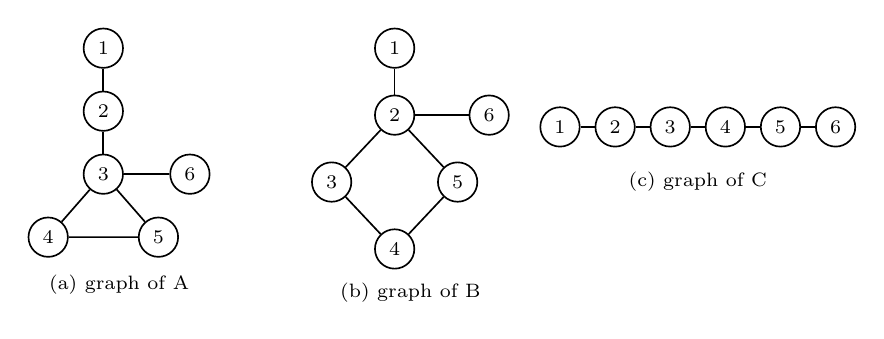
\begin{tikzpicture}[
   vtx/.style={circle,draw,semithick,fill=white,minimum size=5mm,inner sep=0pt,font=\scriptsize},
   every path/.style={semithick}]
  % A: 3-node loop
  \node[vtx](a1) at (0,0){1};   \node[vtx](a2) at (0,-0.8){2};
  \node[vtx](a3) at (0,-1.6){3}; \node[vtx](a6) at (1.1,-1.6){6};
  \node[vtx](a4) at (-0.7,-2.4){4}; \node[vtx](a5) at (0.7,-2.4){5};
  \draw (a1)--(a2)--(a3); \draw (a3)--(a4)--(a5)--(a3); \draw (a3)--(a6);
  \node[font=\scriptsize] at (0.2,-3.0){(a) graph of A};
  % B: 4-node loop (diamond)
  \begin{scope}[xshift=37mm]
    \node[vtx](b1) at (0,0){1};      \node[vtx](b2) at (0,-0.85){2};
    \node[vtx](b6) at (1.2,-0.85){6};
    \node[vtx](b3) at (-0.8,-1.7){3}; \node[vtx](b5) at (0.8,-1.7){5};
    \node[vtx](b4) at (0,-2.55){4};
    \draw (b1)--(b2); \draw (b2)--(b6); \draw (b2)--(b3)--(b4)--(b5)--(b2);
    \node[font=\scriptsize] at (0.2,-3.1){(b) graph of B};
  \end{scope}
  % C: horizontal chain (no loop)
  \begin{scope}[xshift=58mm, yshift=-1.0cm]
    \node[vtx](c1) at (0,0){1};   \node[vtx](c2) at (0.7,0){2};
    \node[vtx](c3) at (1.4,0){3}; \node[vtx](c4) at (2.1,0){4};
    \node[vtx](c5) at (2.8,0){5}; \node[vtx](c6) at (3.5,0){6};
    \draw (c1)--(c2)--(c3)--(c4)--(c5)--(c6);
    \node[font=\scriptsize] at (1.75,-0.7){(c) graph of C};
  \end{scope}
\end{tikzpicture}
\end{minipage}\hfill
\begin{minipage}[c]{0.27\linewidth}
\centering
% grayscale barcode: darkness = lambda / lambda_max, lambda_max = 5.236
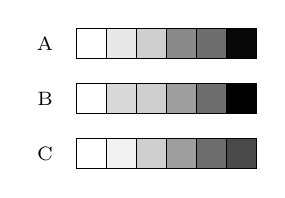
\begin{tikzpicture}[every path/.style={thin}]
  \def\cw{0.38}
  \node[font=\scriptsize] at (-0.4,0)    {A};
  \foreach \i/\p in {0/0,1/9,2/19,3/46,4/57,5/97}
     {\fill[black!\p] (\i*\cw,-0.19) rectangle ++(\cw,0.38);
      \draw (\i*\cw,-0.19) rectangle ++(\cw,0.38);}
  \node[font=\scriptsize] at (-0.4,-0.7) {B};
  \foreach \i/\p in {0/0,1/15,2/19,3/38,4/57,5/100}
     {\fill[black!\p] (\i*\cw,-0.89) rectangle ++(\cw,0.38);
      \draw (\i*\cw,-0.89) rectangle ++(\cw,0.38);}
  \node[font=\scriptsize] at (-0.4,-1.4) {C};
  \foreach \i/\p in {0/0,1/5,2/19,3/38,4/57,5/71}
     {\fill[black!\p] (\i*\cw,-1.59) rectangle ++(\cw,0.38);
      \draw (\i*\cw,-1.59) rectangle ++(\cw,0.38);}
\end{tikzpicture}\\[2pt]
{\scriptsize spectrum as a barcode\\(each cell $=\lambda_i$, darker $=$ larger)}
\end{minipage}

\caption{Three Java fragments, their graphs, and their spectra as a
grayscale barcode. A and B both sum an array and are clones, but A has a
three-node loop and B a four-node loop, so their graphs differ. Their
barcodes still look almost the same, while the unrelated function C, which
has no loop, is lighter in the last cell.}
\label{fig:motivating_exp}
\end{figure*}

\autoref{fig:motivating_exp} shows two Java functions that sum an integer
array using different loops and variable names, alongside an unrelated
function C that computes a triangle area. A and B share no identifiers, so
token- and line-based comparison finds little in common
\cite{roy2007survey,alomari2020semanticclonebench}, and their graphs differ
as well: A has a three-node loop, B a four-node loop. Their sorted Laplacian
spectra nonetheless nearly coincide,
$\{0,\,0.485,\,1.000,\,2.425,\,3.000,\,5.089\}$ against
$\{0,\,0.763,\,1.000,\,2.000,\,3.000,\,5.236\}$, whereas C gives
$\{0,\,0.268,\,1.000,\,2.000,\,3.000,\,3.732\}$ with a visibly smaller
leading eigenvalue. Euclidean distance between sorted spectra is $0.53$ for
the clone pair and $1.44$ and $1.58$ for the non-clone pairs, so a single
threshold separates them. Being invariant to relabelling and stable under
small edits, the spectrum matches behaviourally equivalent code that differs
on the surface. {That separation, however, depends entirely on the graph
that was drawn, and no fixed construction guarantees so favourable an
arrangement in general. The question is therefore not which predefined graph
yields the most informative spectrum, but whether the graph itself can be
learned from clone supervision.}

\subsection{Contributions}
\label{subsec:contributions}
The main contributions of this paper are as follows:

\begin{itemize}
    \item \textbf{A Latent Graph Learning Network for Spectral Code Representation}: We propose a Siamese latent-graph network with soft slot assignment and multi-head attention that learns a fixed-size weighted latent graph and derives a multi-scale spectral representation from its normalized Laplacian, substantially improving spectral discriminative power over conventional program graphs.

    \item \textbf{Comprehensive Comparison with Semantic CCD Baselines}: We compare our approach with state-of-the-art non-graph, graph-based, hybrid graph--code, and pretrained approaches across diverse single-language and cross-language benchmarks, demonstrating improved semantic clone detection performance across multiple evaluation settings.

    \item \textbf{Cross-Dataset and Cross-Language Generalization}: We systematically analyze the generalization power of \method{} across dataset and language boundaries under strict leakage-free evaluation, providing a rigorous assessment of its generalizability beyond conventional within-dataset settings.
\end{itemize}
% For Mohsen to write the first-version

% Proposing a new graph design for source codes that gives us a good spectral representation --> (a) better than AST, CFG, PDG, DDG, etc (traditional graph representations) judged over code clone benchmarks and how good we score. Also, (b) further analysis and backing of the good graph design made by us.

% Empirical study and Exploration of spectral representation over "different graphs of code" on "diverse set of datasets" in "both single-language and cross-language" compared with "Statistical Token based feature space" and "CodeBert Transformer-type embeddings" and "various other CCD approaches that are trained (not baseline but previous work)" using "different metrics" and "eigenvalue + eigenvector" through "other variable and experiments".

% Analytical and a thorough investigation of spectral representation space of source codes and insights and projection operators over that space. --> Eigenvectors and how they can be used for spectral representations in general.


\subsection{Paper Organization}
\label{subsec:outline}

The rest of this paper is organized as follows. \autoref{sec:related_work} reviews related work on code clone
detection, source code representation, spectral analysis of graphs, {and latent graph learning}. We then present our
latent graph induction and spectral representation, followed by the experimental setup and the results on single-language and cross-language benchmarks. Finally, we analyze the spectral representation space and conclude with a summary and directions for future work.


\section{Related Work}
\label{sec:related_work}

% Our work builds on four lines of research: code clone detection, source
% code representation, spectral analysis of graphs, and latent graph
% learning. We first review how clone detection has
% moved from text and token matching to learning and graph based semantic
% methods (\autoref{subsec:ccd}). We then describe how source code is
% encoded into the structural and learned representations that detectors
% rely on (\autoref{subsec:representation}). After that we summarise the
% theory and the main applications of graph spectral analysis in other
% fields (\autoref{subsec:spectral}). This last part motivates our use
% of the graph spectrum as a signature of code structure that does not
% depend on node ordering. We then review latent graph learning, which
% supplies the mechanism for inducing the graph on which that spectrum is
% computed (\autoref{subsec:latent_graph}). We close by positioning our
% contribution against this body of work (\autoref{subsec:gap}).

% ---------------------------------------------------------------------
\subsection{Code Clone Detection}
\label{subsec:ccd}

Code clone detection has been studied for more than two decades. Most
techniques are grouped by the program representation on which similarity
is measured. Roy and Cordy \cite{roy2007survey} classify clones into four
types. Type-1 clones are identical except for formatting and naming.
Type-2 and Type-3 clones are syntactically similar but contain small
changes. Type-4 clones implement the same functionality with different
syntax.

\textbf{Text and token based approaches.} The earliest scalable detectors
work on lexical information. \emph{CCFinder} \cite{kamiya2002ccfinder}
normalises token sequences and compares them across several languages.
Working at line granularity instead, Ducasse et al.\
\cite{ducasse1999language} detect duplicated code in a language independent
way, while \emph{CP-Miner} \cite{li2006cpminer} mines copy-paste bugs in
large systems. \emph{NICAD} \cite{roy2008nicad} adds flexible
pretty-printing to line based comparison, which lets it capture near-miss
clones. Scaling to very large code bases required indexing and filtering.
Three strategies stand out here: an inverted index in \emph{SourcererCC}
\cite{sajnani2016sourcerercc}, overlapping code windows in
\emph{CCAligner} \cite{wang2018ccaligner}, and metric based filtering in
\emph{Oreo} \cite{saini2018oreo}. A more recent detector,
\emph{StoneDetector} \cite{heinze2025stonedetector}, compares paths taken
from dominator trees of Java source and bytecode. All of these methods
scale well. They mostly ignore code structure, however, so they have
trouble with Type-3 and Type-4 clones.

\textbf{Tree and graph based approaches.} To capture structural
similarity, detectors began to use the abstract syntax tree (AST).
Baxter et al.\ \cite{baxter1998clone} match subtrees of the AST.
\emph{DECKARD} \cite{jiang2007deckard} describes subtrees with numerical
vectors and clusters them in Euclidean space. Some clones survive
statement reordering or interleaving, which lexical and tree methods miss.
This motivated graph based detectors. Komondoor and Horwitz
\cite{komondoor2001slicing} and Krinke \cite{krinke2001identifying} search
for isomorphic subgraphs of the program dependence graph (PDG). The PDG
uses control flow and data flow rather than surface syntax. Subgraph
isomorphism is expensive to compute, which has limited the scalability of
PDG based methods.

\textbf{Learning and deep learning based approaches.} A large body of
recent work learns similarity directly from data. White et al.\
\cite{white2016deep} were among the first to apply deep learning to clone
detection. They link lexical patterns with syntactic patterns. The
\emph{CDLH} framework \cite{wei2017cdlh} treats functional clone detection
as a supervised hashing problem over AST based LSTMs. \emph{ASTNN}
\cite{zhang2019astnn} splits an AST into statement subtrees and encodes
them with recurrent networks. Tree based convolution
\cite{yu2019neural} and recursive aggregation of ASTs
\cite{buch2019learning} are other structural encoders. Graph neural
networks (GNNs) reduce the semantic gap further. The flow augmented AST
(\emph{FA-AST}) of Wang et al.\ \cite{wang2020faast} adds control flow and
data flow edges to the AST and applies GNNs to measure pairwise
similarity. Graph based semantics learning \cite{yu2023graphsemantics}
combines CFG and PDG representations with attention based graph matching.
\emph{FSD-CLCD} \cite{zhang2024fsdclcd} addresses cross-language detection
through functional semantic distillation over AST derived graphs. Other
work targets efficiency. Transformer based detectors with code token
learners \cite{zhang2023efficient} reduce the cost of attention.
\emph{CCStokener} \cite{wang2023ccstokener} adds semantic information to
tokens. \emph{Code2Img} \cite{hu2023code2img} turns the AST adjacency
matrix into an image and processes it with convolutional networks. The
\emph{BigCloneBench} benchmark \cite{svajlenko2014bigclonebench} is the
standard dataset for evaluating these detectors at scale.

These detectors are accurate but carry practical costs. GNN and Transformer
based methods need large labelled datasets, rely on costly pairwise
comparison, and are expensive to train. Their learned similarity is also
sensitive to node ordering and to graph size. \added{The graph or token view is also fixed
before training. A detector can then exploit only those relations the chosen
view already exposes. These limitations motivate representations of code
structure that are compact, invariant to node ordering, and not tied to a
program graph selected beforehand.}

% ---------------------------------------------------------------------
\subsection{Source Code Representation}
\label{subsec:representation}

The performance of a clone detector depends heavily on how source code is
represented. The classical representations are explicit program structures:
the AST captures syntax, while the control flow graph (CFG) and the PDG
capture execution and dependence relations. The code property graph (CPG) of
Yamaguchi et al.\ \cite{yamaguchi2014cpg} joins syntax, control flow, and data
flow in a single graph and has proven effective for finding vulnerabilities.
These graph representations retain rich semantic information, but they are
high dimensional and irregular, which makes direct comparison difficult.
\added{They also differ in what they suppress, so choosing among them is a
modelling assumption rather than a neutral preprocessing step.}

A second line of work learns continuous representations of code.
\emph{code2vec} \cite{alon2019code2vec} aggregates AST paths into a fixed
length embedding that predicts semantic properties of a snippet.
Pre-trained language models extend this idea to large corpora:
\emph{CodeBERT} \cite{feng2020codebert} learns joint representations of
programming language and natural language, and \emph{GraphCodeBERT}
\cite{guo2021graphcodebert} adds data flow structure to the pre-training
objective, improving downstream tasks such as clone detection.
Structure aware neural encoders such as ASTNN \cite{zhang2019astnn} and
FA-AST \cite{wang2020faast} can also be read as representation learners.
These embeddings are powerful, but they are learned end to end, they depend on
their training distribution, and they are hard to interpret. \added{In every case the input
view is given. The encoder learns what to compute over the AST or data flow
graph, not which relational structure to compute it over. Our work retains
supervised learning but moves that decision inside the model. The representation
is derived from the algebraic structure of a graph induced under clone
supervision.}

% ---------------------------------------------------------------------
\subsection{Spectral Analysis of Graphs}
\label{subsec:spectral}

Spectral graph theory studies a graph through the eigenvalues and eigenvectors
of its adjacency matrix and Laplacian \cite{chung1997spectral,mohar1991laplacian}.
The spectrum encodes global structure: Fiedler showed that the second smallest
Laplacian eigenvalue measures connectivity \cite{fiedler1973algebraic}. Because
eigenvalues are unchanged by relabelling, the spectrum is a natural signature
for comparing graphs of different sizes, the property that AST and PDG
comparison requires. The same eigenbasis underlies spectral clustering
\cite{shi2000normalized,ng2002spectral,vonluxburg2007tutorial}, Laplacian
eigenmaps \cite{belkin2003laplacian}, spectral correspondence
\cite{leordeanu2005spectral}, and isometry-invariant shape descriptors such as
the heat kernel signature \cite{sun2009hks,zhang2010spectralmesh}. Graph kernels
compare structures by iterative refinement \cite{shervashidze2011wl}, and
spectral convolution defines modern graph deep learning
\cite{bruna2014spectral,defferrard2016cnngraph,kipf2017gcn}, later generalised
by attention \cite{velickovic2018gat}. \added{Across these applications the
graph is given by the data or built by a domain-specific rule, and that
construction bounds the descriptor.} Spectral signatures of code graphs,
meanwhile, have received little attention in clone detection.

% ---------------------------------------------------------------------
\subsection{Latent Graph Learning}
\label{subsec:latent_graph}

\added{Message-passing networks assume the graph is given, which is a source of
error when it is unavailable or only loosely related to the task. Latent graph
learning, also studied as graph structure learning, instead treats the adjacency
as a latent variable estimated jointly with the predictor \cite{zhu2021gslsurvey}.
Neural relational inference recovers interaction structure from trajectories via
a latent edge posterior \cite{kipf2018nri}; LDS learns a discrete distribution
over graphs by bilevel optimization of the downstream loss
\cite{franceschi2019lds}; IDGL alternates between refining embeddings and
re-estimating a similarity graph \cite{chen2020idgl}; and differentiable
generators let each node choose its neighbours and their number
\cite{saha2023adaptive}. Learned coarsening is complementary: DiffPool maps nodes
to a fixed number of clusters through a soft assignment matrix, yielding graphs
whose size is independent of the input \cite{ying2018diffpool}.}

\added{Both mechanisms fit clone detection, where the program graph is normally
fixed before training and each view suppresses some relations
\cite{yamaguchi2014cpg}, a bias inherited by existing detectors
\cite{wang2020faast,yu2023graphsemantics,zhang2024fsdclcd}. They also suit
spectral analysis: a constant number of latent nodes makes Laplacian spectra
comparable across fragments of very different length, and a real-valued
differentiable adjacency allows spectral quantities to be optimized end to end.
Software engineering has so far modified code graphs by rule rather than by
learning, as when AMPLE merges syntax nodes and fuses edge types before message
passing \cite{wen2023ample}, so the graph remains a preprocessing choice. We are
not aware of prior work that fits the adjacency underlying a code representation
to the detection objective, or computes a spectral descriptor on such a graph.}

% % ---------------------------------------------------------------------
% \subsection{Positioning of Our Work}
% \label{subsec:gap}

% Token and tree based detectors scale well but miss semantic clones. GNN and
% Transformer based detectors capture semantics at the cost of large labelled
% corpora and expensive training, and remain sensitive to graph size and node
% ordering. Spectral analysis gives a compact, permutation-invariant description
% of global structure, but a spectrum computed from an unsuitable program graph
% discards task-relevant semantics. \added{We therefore combine spectral
% description with latent graph learning rather than treating either alone as
% sufficient. The latent graph is learnable, clone supervision determines its
% topology, and a multi-scale spectral descriptor is computed on the induced
% graph. Fixed-graph spectral methods and observed-graph GNNs are retained as
% controls, so the experiments can separate the contribution of spectral
% comparison from that of task-guided graph induction.}


\section{Methodology}
\label{sec:revised_methodology}

Spectral representations provide compact, permutation-invariant descriptions of graph structure and have been used for graph comparison and matching \cite{wilson2008study}. Their discriminative content, however, depends on the graph being represented. Using a fixed AST, CFG, or DDG therefore commits the representation to a predefined structural view of the program. We instead learn a latent graph from semantic-clone supervision and optimize it jointly with the downstream prediction task \cite{yu2021deep}.

\subsection{Problem Formulation}
\label{sec:revised_problem_formulation}

Let $\mathcal{L}$ denote a set of programming languages, $\mathcal{C}_{\ell}$ the set of code fragments written in language $\ell\in\mathcal{L}$, and $\mathcal{C}=\bigcup_{\ell\in\mathcal{L}}\mathcal{C}_{\ell}$. Given a labeled training set $\mathcal{D}_{\mathrm{tr}}=\{(c_i,c_j,y_{ij})\}$, where $c_i,c_j\in\mathcal{C}$,
\begin{equation}
y_{ij}=
\begin{cases}
1, & c_i\equiv_{\mathrm{func}}c_j,\\
0, & \text{otherwise},
\end{cases}
\label{eq:revised_clone_label}
\end{equation}
indicates whether the two fragments implement the same functionality. Let $\mathcal{G}_{m,d}$ denote the space of weighted attributed graphs with $m$ latent nodes, each represented by a $d$-dimensional feature vector. We seek a parameterized code-to-graph mapping $G_{\Theta}:\mathcal{C}\rightarrow\mathcal{G}_{m,d}$ such that $G_{\Theta}(c)=(Z_{\Theta}(c),A_{\Theta}(c))$. The graph is represented by its spectral signature $s_{\Theta}(c)=\operatorname{Spec}(G_{\Theta}(c))\in\mathbb{R}^{d_s}$. Define
\begin{equation}
S_{\Theta}(c_i,c_j)
=
\cos\!\left(s_{\Theta}(c_i),s_{\Theta}(c_j)\right).
\label{eq:spectral_similarity_old}
\end{equation}
and let the spectral loss be
\begin{equation}
\ell_{ij}(\Theta)
=
y_{ij}(1-S_{\Theta}(c_i,c_j))
+
(1-y_{ij})[S_{\Theta}(c_i,c_j)-\mu_{\mathrm{spec}}]_{+},
\label{eq:spectral_loss_old}
\end{equation}
where $[x]_{+}=\max(0,x)$ and $\mu_{\mathrm{spec}}\in[0,1)$ is the negative-pair similarity margin, specifying the maximum similarity tolerated for negative pairs. The objective then is to learn $g_{\Theta}$ such that functional equivalence is preserved in the induced spectral space, i.e.,
\begin{equation}
\Theta^{*}
=
\arg\min_{\Theta}
\mathbb{E}_{(c_i,c_j,y_{ij})\sim\mathcal{D}_{\mathrm{tr}}}
\left[\ell_{ij}(\Theta)\right].
\label{eq:latent_graph_objective_old}
\end{equation}
At inference time, the complete model produces a clone probability $\widehat{p}_{ij}$ for each pair. Clone detection is performed as $\widehat{y}_{ij}=\mathbb{I}[S_{\Theta^{*}}(c_i,c_j)\geq\gamma]$, where $\gamma$ is the decision threshold.

\subsection{\method{}}
\label{sec:revised_spectra_siam}

\method{} uses a Siamese architecture with shared parameters for the two code fragments \cite{bromley1993signature}. Each branch constructs a normalized attributed program graph and encodes its syntactic and data-dependence relations. It then maps the variable-size graph to a fixed set of latent nodes to learn their weighted adjacency and derives a multi-scale spectral representation. Spectral features are then compared by a pairwise classifier to output a prediction in $[0,1]$. \autoref{fig:spectra_overview} summarizes the pipeline.

\begin{figure*}[t]
    \centering
    \safeincludegraphics[width=1.0\textwidth]{figures/main_fig.png}
    \caption{\method{} architecture.}
    \label{fig:spectra_overview}
\end{figure*}


\subsubsection{Stage 1: Initial representation and Language Normalization}
\label{sec:revised_input_representation}

Each code fragment is first converted into an attributed graph whose nodes have numerical representations and whose edges encode structural relations. Combining syntactic structure with semantic or data-flow relations is common in learned program representations \cite{allamanis2018learning,yamaguchi2014cpg}. We use AST to provide the node backbone and augment it with DDG edges whose endpoints can both be mapped to AST nodes. The edges are made bidirectional before batching.

\paragraph{Canonical node types}
Parser node names vary across languages and extraction tools, so raw types are mapped to a shared vocabulary $\mathcal{K}_{\mathrm{can}}$:
\begin{quote}\scriptsize
Control\_If, Control\_Loop, Control\_Switch, Control\_Return,
Control\_Break, Control\_Generic, Var\_Decl, Func\_Decl,
Class\_Decl, Param\_Decl, Assign\_Op, Binary\_Op, Unary\_Op,
Call\_Expr, Access\_Expr, Literal\_Num, Literal\_Str,
Literal\_Bool, Literal\_Null, Literal\_Generic, Structural\_Block,
Identifier\_Context, Type\_Meta, and Canonical\_Unknown.
\end{quote}
The mapping covers \texttt{Joern}, Python's AST parser, and the language-specific parser fallbacks used in preprocessing; unmatched types are assigned to \texttt{Canonical\_Unknown}.

\paragraph{Hashed lexical features}
The canonical type alone does not preserve all information carried by the original node label. We therefore keep a small amount of lexical information for each node. Non-numeric labels are split at punctuation and camel-case boundaries~\cite{hill2014empirical}, and literals are normalized. The resulting sub-tokens, together with their character $n_{\mathrm{char}}$-grams, are mapped by a deterministic hash function to $N_{\mathrm{hash}}$ indices \cite{weinberger2009feature}. This keeps the lexical vocabulary at a fixed size regardless of the source language or dataset. We keep at most $r_{\max}$ lexical features per node and ignore labels that contain only line numbers. For node $v$, let $\kappa(t_v)$ be its canonical type and $\ell_{v1},\ldots,\ell_{vr}$ its lexical features. We combine the embedding of the canonical type with the average embedding of these lexical features:
\begin{equation}
h_v^{(0)}
=
\operatorname{LN}\!\left(
E_{\mathrm{can}}(\kappa(t_v))
+
\gamma_{\mathrm{lex}}
\frac{1}{r}
\sum_{q=1}^{r}
E_{\mathrm{lex}}(\ell_{vq})
\right),
\
\gamma_{\mathrm{lex}}=\sigma(g_{\mathrm{lex}}).
\label{eq:revised_node_initialization_old}
\end{equation}
where $E_{\mathrm{can}}$ and $E_{\mathrm{lex}}$ are learned embedding tables. The learned scalar $\gamma_{\mathrm{lex}}\in(0,1)$ controls how strongly the lexical information contributes to the initial node representation. Layer normalization and dropout are applied to the lexical features during
training to improve numerical stability and provide regularization
\cite{ba2016layer,srivastava2014dropout}. Graphs are restricted to the first $n_{\max}$ serialized AST nodes; padding is excluded from message passing and reconstruction.



\subsubsection{Stage 2: Relation-Aware Structural Encoding}
\label{sec:revised_relation_encoder}

AST and DDG edges represent different relations and should therefore use separate transformations~\cite{schlichtkrull2018modeling}. Let $H^{(l)}\in\mathbb{R}^{n\times d}$ contain node states at layer $l$ and $A^{(r)}$ denote the adjacency for relation $r\in\mathcal{R}$. Each layer computes
\begin{equation}
\begin{aligned}
U^{(l)}
&=
H^{(l)}W_0^{(l)}
+
\sum_{r\in\mathcal{R}}
\widetilde{A}^{(r)}H^{(l)}W_r^{(l)},\\
H^{(l+1)}
&=
\operatorname{LN}\!\left[
H^{(l)}
+
\operatorname{Dropout}
\bigl(\operatorname{GELU}(U^{(l)})\bigr)
\right],
\end{aligned}
\label{eq:revised_relation_layer}
\end{equation}
where $\widetilde{A}^{(r)}$ is row-normalized, with a minimum degree denominator of one. $W_0^{(l)}$ transforms the current state and $W_r^{(l)}$ is relation specific. The residual, normalization, GELU, and dropout components follow standard
formulations \cite{he2016deep,ba2016layer,hendrycks2016gaussian,srivastava2014dropout}. The encoder uses $L_{\mathrm{enc}}$ layers of dimension $d$.


\subsubsection{Stage 3: Latent Graph Induction}
\label{sec:revised_latent_induction}

We reduce the number of node states to $m$ latent nodes using iterative soft
assignment, following the general idea of differentiable graph pooling
\cite{ying2018hierarchical}. For normalized input key $k_v$ and latent query $q_j$,
\begin{equation}
P_{vj}
=
\frac{\exp(q_j^{\top}k_v/\sqrt{d})}
{\sum_{u=1}^{m}\exp(q_u^{\top}k_v/\sqrt{d})}.
\label{eq:revised_slot_assignment}
\end{equation}
Latent updates normalize contributions over valid input nodes and use a GRU followed by a residual MLP \cite{cho2014gru,he2016resnet}. After $I_{\mathrm{assign}}$ iterations, the latent states form $Z\in\mathbb{R}^{m\times d}$. To limit information loss during pooling, $\widehat{H}=PZ$ reconstructs the input states. With $M_v$ indicating valid nodes,
\begin{equation}
\mathcal{L}_{\mathrm{rec}}
=
\frac{1}{\sum_v M_v}
\sum_v
M_v
\frac{1}{d}
\left\|
h_v^{(0)}-\widehat{h}_v
\right\|_2^2.
\label{eq:revised_reconstruction_loss}
\end{equation}

The observed structure is projected into latent space as
\begin{equation}
B=P^{\top}A_{\mathrm{in}}P,
\qquad
\widetilde{B}
=
\frac{B}{\max_{i,j}B_{ij}+\epsilon},
\label{eq:revised_structure_projection}
\end{equation}
where $A_{\mathrm{in}}$ combines the enabled input relations and $\widetilde{B}$ serves as a prior. Task-dependent affinities are obtained from $H_a$ scaled dot-product attention heads~\cite{vaswani2017attention}:
\begin{equation}
S
=
\operatorname{Sym}\!\left(
\frac{1}{H_a}
\sum_{h=1}^{H_a}
\frac{Q_hK_h^{\top}}{\sqrt{d_h}}
\right)
+
\eta\widetilde{B},
\label{eq:revised_latent_affinity}
\end{equation}
where $\eta$ learns the contribution of the projected AST/DDG
structure. Thus, the latent topology combines observed structure with task-
dependent affinities, following the general setting of graph structure learning
\cite{jin2020graph}.

\paragraph{Adaptive edge temperature}
We convert $S$ to continuous edge weights using a temperature conditioned on graph size and density. For $n(c)$ valid nodes, define node occupancy $u(c)=n(c)/n_{\max}$ and
$\rho_{\mathrm{in}}(c)=\operatorname{clip}_{[0,1]}(\sum_{r,i,j}A_{ij}^{(r)}/n(c)^2)$.
Their mixture is
$\chi(c)=\beta_u u(c)+(1-\beta_u)\rho_{\mathrm{in}}(c)$, giving
\begin{equation}
T(c)
=
T_{\min}
+
(T_{\max}-T_{\min})
\sigma\!\left(
b_T+\operatorname{softplus}(w_T)\chi(c)
\right).
\label{eq:revised_adaptive_temperature}
\end{equation}
After clipping $S$ to $[-s_{\max},s_{\max}]$, the latent adjacency is
\begin{equation}
A_{\Theta}(c)
=
\operatorname{Sym}\!\left[
\sigma\!\left(\frac{S}{T(c)}\right)
\odot
(\mathbf{1}\mathbf{1}^{\top}-I_m)
\right].
\label{eq:revised_latent_adjacency}
\end{equation}
$A_{\Theta}(c)$ is symmetric, continuous, and zero-diagonal; no hard edge threshold is applied. $L_{\mathrm{ref}}$ additional graph layers refine $Z$ using this learned adjacency. \autoref{fig:latent_graph_induction} summarizes
the complete latent-graph induction process.

\begin{figure}[t]
    \centering
    \safeincludegraphics[width=1.0\columnwidth]{figures/latent_graph_induction.png}
    \caption{
    Latent graph induction in \method{}.
    }
    \label{fig:latent_graph_induction}
\end{figure}

\subsubsection{Stage 4: Multi-Scale Spectral Representation}
\label{sec:revised_multiscale_spectrum}
The learned graph and its latent-node attributes are summarized jointly through an attributed graph-spectral representation. We first construct the normalized Laplacian
\begin{equation}
L_{\Theta}
=
I_m-D_{\Theta}^{-1/2}A_{\Theta}D_{\Theta}^{-1/2},
\qquad
D_{\Theta}
=
\operatorname{diag}(A_{\Theta}\mathbf{1}),
\label{eq:revised_normalized_laplacian}
\end{equation}
wwhose eigenvalues lie in $[0,2]$ for an undirected graph with non-negative
edge weights \cite{chung1997spectral}. A small deterministic diagonal perturbation up to $\epsilon_{\mathrm{eig}}$ is added before eigen-decomposition to improve numerical stability. We then combine three complementary spectral summaries.

\paragraph{Eigenvalue density}
For normalized Laplacian eigenvalues
$\lambda_1,\ldots,\lambda_m$, a Gaussian-smoothed profile
\cite{banerjee2008spectrum,lewitus2016characterizing} is evaluated at
$N_\xi$ centers $\xi_j\in[0,2]$:
\begin{equation}
d_j
=
\frac{1}{m}
\sum_{i=1}^{m}
\exp\!\left[
-\frac{1}{2}
\left(
\frac{\lambda_i-\xi_j}{\sigma_{\mathrm{dens}}}
\right)^2
\right],
\quad
j=1,\ldots,N_{\xi},
\label{eq:revised_eigenvalue_density}
\end{equation}
giving $d(c)\in\mathbb{R}^{N_{\xi}}$.

\paragraph{Heat traces}
Heat diffusion captures structure across scales
\cite{sun2009concise}. At logarithmically spaced $t_q\in[t_{\min},t_{\max}]$,
\begin{equation}
h_q
=
\frac{1}{m}
\sum_{i=1}^{m}
\exp(-t_q\lambda_i),
\qquad
q=1,\ldots,N_t,
\label{eq:revised_heat_trace}
\end{equation}
yielding $h(c)\in\mathbb{R}^{N_t}$.

\paragraph{Graph-signal Chebyshev energies}
To preserve information about node attributes within the spectral representation, the refined latent states $Z$ are projected to $N_{\mathrm{sig}}$ graph-signal channels:
\begin{equation}
\widetilde{X}
=
ZW_s
\in\mathbb{R}^{m\times N_{\mathrm{sig}}}.
\label{eq:revised_raw_graph_signal}
\end{equation}
The signals are RMS-normalized across latent nodes:
\begin{equation}
X_{vr}
=
\frac{\widetilde{X}_{vr}}
{
\sqrt{
\frac{1}{m}
\sum_{u=1}^{m}
\widetilde{X}_{ur}^{\,2}
+\epsilon
}
},
\qquad
r=1,\ldots,N_{\mathrm{sig}}.
\label{eq:revised_graph_signal}
\end{equation}
This normalization removes signal-scale effects before spectral filtering~\cite{??}. Since the normalized-Laplacian spectrum lies in $[0,2]$, we use $\widetilde{L}=L_{\Theta}-I_m$ and the Chebyshev recurrence
\begin{equation}
T_0(X)=X,\quad
T_1(X)=\widetilde{L}X,\quad
T_k(X)=2\widetilde{L}T_{k-1}(X)-T_{k-2}(X).
\end{equation}
Chebyshev approximations allow spectral filtering without explicit eigenvector multiplication \cite{defferrard2016chebnet}. For $N_{\mathrm{band}}$ Gaussian filters,
\begin{equation}
Y_b
=
\sum_{k=0}^{K_{\mathrm{cheb}}}
a_{bk}T_k(X),
\qquad
b=1,\ldots,N_{\mathrm{band}},
\label{eq:revised_chebyshev_filter}
\end{equation}
where the filter centers lie in $[\omega_{\min},\omega_{\max}]$ with bandwidth $\sigma_{\mathrm{filt}}$ and fixed coefficients $a_{bk}$. The graph-signal readout uses fixed, uniformly weighted bands; it does not use a state-conditioned attention gate. For signal channel $r$ and band $b$,
\begin{equation}
e_{br}
=
\frac{1}{m}
\sum_{i=1}^{m}
Y_b(i,r)^2.
\label{eq:revised_spectral_energy}
\end{equation}
Thus $e(c)\in\mathbb{R}^{N_{\mathrm{band}}N_{\mathrm{sig}}}$, and the complete descriptor is
\begin{equation}
s_{\Theta}(c)
=
d(c)\concat h(c)\concat e(c)
\in\mathbb{R}^{d_s},
\
d_s
=
N_{\xi}+N_t+N_{\mathrm{band}}N_{\mathrm{sig}}.
\label{eq:revised_spectral_descriptor}
\end{equation}
All three descriptors are derived from the learned latent adjacency. The Chebyshev path propagates supervision through the learned adjacency and graph-signal projection; no pooled node state or raw lexical vector is concatenated to the classifier input.

\subsubsection{Separate Block-wise Spectral Comparison}
\label{sec:revised_head}
Let $\mathcal{S}=\{d,h,e\}$ denote the density, heat-trace, and Chebyshev-energy blocks, and let $s_b(c)$ be block $b$ of $s_{\Theta}(c)$. Each block is transformed and normalized separately:
\begin{equation}
u_b(c)=\operatorname{Norm}_2\!\left(\log(1+s_b(c))\right).
\label{eq:revised_block_normalization}
\end{equation}
For pair $(c_i,c_j)$, the classifier receives, for every block independently, the symmetric interactions $|u_b(c_i)-u_b(c_j)|$, $u_b(c_i)\odot u_b(c_j)$, and $|\log(1+s_b(c_i))-\log(1+s_b(c_j))|$, together with its cosine similarity and mean and root-mean-square absolute difference. The concatenation of these block-wise comparisons, denoted $q_{ij}$, is the \emph{only} input to an $L_{\mathrm{pair}}$-layer MLP that produces a scalar logit and sigmoid probability $\widehat{p}_{ij}$. Thus neither an individual descriptor, a code embedding, a pooled latent state, nor a lexical or source-token feature has a direct decision path.

\subsubsection{Training Objective}
\label{sec:revised_training_objective}

Training combines classification, block-wise spectral contrast, batchwise AUC ranking, hard-negative separation, graph and topology reconstruction, variance preservation, and graph regularization.

\paragraph{Classification loss}
With $N_+$ and $N_-$ denoting clone and non-clone training pairs, define $w_+=\min(w_{\max},N_-/\max(1,N_+))$. For mini-batch $\mathcal{B}$,
\begin{equation}
\mathcal{L}_{\mathrm{cls}}
=
-\frac{1}{|\mathcal{B}|}
\sum_{(i,j)\in\mathcal{B}}
\left[
w_+y_{ij}\log\widehat{p}_{ij}
+
(1-y_{ij})\log(1-\widehat{p}_{ij})
\right].
\label{eq:revised_classification_loss}
\end{equation}

\paragraph{Spectral contrastive loss}
For the mean block-wise similarity $c^s_{ij}=|\mathcal{S}|^{-1}\sum_{b\in\mathcal{S}}\cos(u_b(c_i),u_b(c_j))$, contrastive supervision \cite{hadsell2006contrastive} is
\begin{equation}
\mathcal{L}_{\mathrm{spec}}
=
\frac{1}{|\mathcal{B}|}
\sum_{(i,j)\in\mathcal{B}}
\left[
y_{ij}(1-c^s_{ij})^2
+
(1-y_{ij})
\relu{c^s_{ij}-\mu_{\mathrm{spec}}}^{2}
\right].
\label{eq:revised_spectral_contrastive}
\end{equation}

\paragraph{Batchwise ranking loss}
Let $\ell_i^+$ and $\ell_j^-$ be positive- and negative-pair logits in the current mini-batch. The differentiable AUC-ranking surrogate is
\begin{equation}
\mathcal{L}_{\mathrm{rank}}
=
\frac{1}{N_+^{\mathcal B}N_-^{\mathcal B}}
\sum_{i,j}
\operatorname{softplus}\!\left[-(\ell_i^+-\ell_j^-)\right],
\label{eq:revised_auc_ranking}
\end{equation}
and is zero when either class is absent from the mini-batch.

\paragraph{Hard-negative loss} To emphasize confusable non-clones
\cite{wang2022disco}, let $\mathcal{K}$ index the
$\max(1,\lfloor\kappa_{\mathrm{hard}}N_-^{\mathcal{B}}\rfloor)$ largest negative-pair values of
$\relu{c^s_{ij}-\mu_{\mathrm{hard}}}^{2}$. Then
\begin{equation}
\mathcal{L}_{\mathrm{hard}}
=
\frac{1}{|\mathcal{K}|}
\sum_{(i,j)\in\mathcal{K}}
\relu{
c^s_{ij}-\mu_{\mathrm{hard}}
}^{2}.
\label{eq:revised_hard_negative}
\end{equation}

\paragraph{Graph regularization}
For a batch of latent adjacencies, let
\begin{equation}
\bar{a}(A)
=
\frac{
\sum_{b=1}^{|\mathcal{B}|}\sum_{i\neq j}A_{b,ij}
}{
|\mathcal{B}|m(m-1)
},
\qquad
\mathcal{L}_{\mathrm{den}}
=
\bigl(\bar{a}(A)-\bar{a}_0\bigr)^2.
\end{equation}
We also record a connectivity term based on the second-smallest Laplacian eigenvalue, i.e., algebraic connectivity \cite{fiedler1973algebraic}:
\begin{equation}
\mathcal{L}_{\mathrm{conn}}
=
\frac{1}{|\mathcal{B}|}
\sum_b
\relu{\mu_{\mathrm{conn}}-\lambda_2^{(b)}}^2,
\qquad
\mathcal{L}_{\mathrm{graph}}
=
\alpha_{\mathrm{den}}\mathcal{L}_{\mathrm{den}}
+
\alpha_{\mathrm{conn}}\mathcal{L}_{\mathrm{conn}}.
\label{eq:revised_graph_regularizer}
\end{equation}
Spectral operations are evaluated in single precision as functions of the learned latent adjacency.

The remaining auxiliary terms are graph reconstruction $\mathcal{L}_{\mathrm{rec}}$, observed-topology reconstruction $\mathcal{L}_{\mathrm{topo}}$, and a spectral-variance floor $\mathcal{L}_{\mathrm{var}}$ that discourages descriptor collapse. The compatibility argument for embedding-level contrast is fixed to zero and any non-zero value is rejected.

The complete objective is
\begin{equation}
\begin{aligned}
\mathcal{L}_{\mathrm{total}}
={}&\mathcal{L}_{\mathrm{cls}}
+\lambda_{\mathrm{spec}}\mathcal{L}_{\mathrm{spec}}
+\lambda_{\mathrm{rank}}\mathcal{L}_{\mathrm{rank}}
+\lambda_{\mathrm{hard}}\mathcal{L}_{\mathrm{hard}}\\
&+\lambda_{\mathrm{rec}}\mathcal{L}_{\mathrm{rec}}
+\lambda_{\mathrm{topo}}\mathcal{L}_{\mathrm{topo}}
+\lambda_{\mathrm{var}}\mathcal{L}_{\mathrm{var}}\\
&+\lambda_{\mathrm{graph}}\mathcal{L}_{\mathrm{graph}}.
\end{aligned}
\label{eq:revised_complete_loss}
\end{equation}

\subsubsection{Optimization}
\label{sec:revised_optimization}

All learnable components are optimized jointly with AdamW \cite{loshchilov2017decoupled}. Neural layers use mixed-precision GPU computation \cite{micikevicius2018mixedprecision}, while latent-adjacency construction and spectral operations use single precision for numerical stability. Numerical hyperparameters are reported in \autoref{tab:revised_spectra_settings}. Checkpoint and decision-threshold selection use only the validation split, as detailed in \autoref{sec:revised_thresholding}.

\section{Experimental Design}
\label{sec:revised_experimental_design}

\subsection{Research Questions}
\label{sec:revised_research_questions}
The objective of this study is to determine whether learning a latent graph can improve spectral code representation for effective and generalizable semantic clone detection. To achieve this objective, we formulate three main research questions as follows:

\begin{itemize}[leftmargin=*]
\item \textbf{RQ1}
\emph{To what extent does the learned graph latent space improve the discriminative power of spectral representations for source code compared with conventional program graphs?}

\item \textbf{RQ2}
\emph{How effective is \method{} compared with state-of-the-art non-graph, graph-based, hybrid graph--code, and pretrained models under conventional evaluation?}

\item \textbf{RQ3}
\emph{How well does \method{} generalize across different semantic CCD datasets and programming languages compared with state-of-the-art models?}

\end{itemize}

\subsection{Dataset}
\label{sec:revised_datasets}
We use three semantic clone datasets: BigCloneBench~\cite{svajlenko2014bigclonebench}, filtered following \cite{wang2020faast}, AtCoder~\cite{perez2019crosslang}, and a new benchmark derived from Project CodeNet~\cite{puri2021codenet}. BigCloneBench contains Java--Java pairs, while AtCoder contains Java--Python pairs. CodeNet covers four within-language configurations (Python--Python, Java--Java, C++--C++, and C\#--C\#) and all six cross-language configurations (Python--Java, Python--C++, Python--C\#, Java--C++, Java--C\#, and C++--C\#) These ten CodeNet configurations are approximately balanced, with about 5K clone pairs targeted per configuration and 50K clone pairs in total. Non-clone pairs are constructed for AtCoder and CodeNet by pairing accepted solutions to different programming problems, following \cite{perez2019crosslang}. \autoref{tab:datasets} summarizes the language configurations, dataset sizes, and train/validation/test splits.

\begin{table}[!htbp]
\centering
\caption{Datasets used in the evaluation. Total and clone counts refer to the complete dataset; train, validation, and test columns report split sizes.}
\label{tab:datasets}

\scriptsize
\renewcommand{\arraystretch}{1.08}
\setlength{\tabcolsep}{2.2pt}

\begin{tabularx}{\columnwidth}{@{}X r r r r r@{}}
\toprule
Dataset & Total & Clones & Train & Val. & Test \\
\midrule

BigCloneBench\cite{svajlenko2014bigclonebench, wang2020faast}
&

&

&

&

&

\\

\quad Java--Java
&
1,731,860
&
561,521
&
901,028
&
415,416
&
415,416
\\

\midrule

AtCoder~\cite{perez2019crosslang}
&

&

&

&

&

\\

\quad Java--Python
&
777,494
&
388,747
&
544,054
&
116,704
&
116,736
\\

\midrule

\textbf{CodeNet}~\cite{puri2021codenet}
&
\textbf{1,949,092}
&
\textbf{961,408}
&
\textbf{1,364,364}
&
\textbf{292,364}
&
\textbf{292,364}
\\

\addlinespace[1pt]

\quad Python--Python
&
194,871
&
94,871
&
136,410
&
29,231
&
29,230
\\

\quad Java--Java
&
195,825
&
95,825
&
137,078
&
29,374
&
29,373
\\

\quad C++--C++
&
197,255
&
97,255
&
138,078
&
29,588
&
29,589
\\

\quad C\#--C\#
&
182,199
&
94,515
&
127,539
&
27,330
&
27,330
\\

\quad Python--Java
&
196,673
&
96,673
&
137,671
&
29,501
&
29,501
\\

\quad Python--C++
&
196,439
&
96,439
&
137,507
&
29,466
&
29,466
\\

\quad Python--C\#
&
195,874
&
95,874
&
137,112
&
29,381
&
29,381
\\

\quad Java--C++
&
196,870
&
96,870
&
137,809
&
29,530
&
29,531
\\

\quad Java--C\#
&
196,115
&
96,115
&
137,280
&
29,417
&
29,418
\\

\quad C++--C\#
&
196,971
&
96,971
&
137,880
&
29,546
&
29,545
\\

\bottomrule
\end{tabularx}
\end{table}
[TO BE REVISED LATER WHEN CODENET IS FINALIZED COMPLETELY]
\paragraph{CodeNet's Clone Extraction Process}
We construct the pairs from CodeNet problem IDs and submission verdicts. Two distinct Accepted submissions to the same problem form a clone. We initially target up to 100K clone pairs for each of the ten language configurations, giving approximately uniform coverage across the four same-language and six cross-language settings. To avoid drawing these pairs mainly from a few popular problems, for each configuration we select up to 500 problems across eight groups based on how many candidate pairs each problem can provide. Within those problems, we sample submissions from different users, submission times, code sizes, and compiler variants. For same-language code, near-duplicates with Jaccard similarity of at least $0.90$ are removed using normalized token shingles and MinHash/LSH \cite{broder1997resemblance,indyk1998ann}; the remaining pairs are selected with preference for less-similar and less-used submissions, and no submission appears in more than 10 clone pairs.

\subsection{Baselines}
\label{sec:revised_baselines}
We compare \method{} with six baseline families: fixed spectral
representations, GNNs over conventional program graphs, non-graph code models, other graph-based models, a hybrid graph--code model, and pretrained code models. For the fixed spectral representations, we consider four downstream settings: no training (\emph{No Train}), Random Forest (RF)~\cite{??}, Logistic Regression (LR)~\cite{??}, and a Siamese Neural Network (SNN)~\cite{??}. Combined with AST, CFG, DDG, and CPG, this gives 16 fixed-spectrum configurations. The GNN~\cite{??} baselines use the same four graph views. We further evaluate Deckard~\cite{??}, RtvNN~\cite{??}, CDLH~\cite{??}, ASTNN~\cite{??}, FA-AST+GGNN~\cite{??}, FA-AST+GMN~\cite{??}, and DeepSim~\cite{??}. Finally, CodeBERT~\cite{??}, GraphCodeBERT~\cite{??}, UniXcoder~\cite{??}, and CodeT5~\cite{??} are evaluated using \emph{No Train}, RF, SNN, Principal Component Analysis (PCA)~\cite{??} followed by RF, and PCA followed by SNN (PCA+SNN). Their main hyperparameters/configurations are summarized in \autoref{tab:revised_baselines}.

\begin{table}[t]
\centering
\caption{Baseline configurations. For neural models, the training column reports batch size / learning rate $\alpha$ / maximum epochs.}
\label{tab:revised_baselines}

\tiny
\renewcommand{\arraystretch}{1.08}
\setlength{\tabcolsep}{1.6pt}

\begin{tabularx}{\columnwidth}{@{}
p{0.19\columnwidth}
p{0.34\columnwidth}
X
r@{}}
\toprule
Method & Input / architecture & Training & Params. \\
\midrule

\multicolumn{4}{@{}l}{\textit{Fixed spectral representations (AST, CFG, DDG, CPG)}} \\[1pt]

No Train
&
72-D spectrum
&
No training
&
0
\\

RF
&
146-D pair features
&
\shortstack[l]{200 trees; depth 16; leaf 5\\
balanced-subsample; seed 42}
&
--
\\

LR
&
146-D pair features
&
\shortstack[l]{train-only scaling; balanced\\
max.\ 1,000 iter.; seed 42}
&
--
\\

SNN
&
$72\!\to\!256\!\to\!256\!\to\!128$
&
\shortstack[l]{$8192/10^{-3}/10$; dropout .10\\
WD $10^{-4}$; clip 5.0}
&
185k
\\

\midrule

\multicolumn{4}{@{}l}{\textit{GNNs over conventional graphs (AST, CFG, DDG, CPG)}} \\[1pt]

GCN
&
\shortstack[l]{5-D nodes; GCN $256/256$; mean pool\\
$128+128+128=384$-D representation}
&
\shortstack[l]{$2048/5{\times}10^{-4}/8$; dropout .05\\
WD $10^{-4}$; patience 3; clip 2.0}
&
989k
\\

\midrule

\multicolumn{4}{@{}l}{\textit{Token, tree, graph, and hybrid baselines}} \\[1pt]

Deckard
&
4,096-D hashed vector; cosine
&
Validation threshold
&
0
\\

RtvNN
&
\shortstack[l]{256 tokens; vocab.\ $\leq50$k; emb.\ 96\\
BiGRU 192; attention; 128-D}
&
\shortstack[l]{$1024/10^{-3}/8$; dropout .15\\
WD $10^{-4}$; patience 2; clip 1.0}
&
1.48--4.46M
\\

CDLH
&
\shortstack[l]{512 tokens; vocab.\ $\leq50$k; emb.\ 128\\
CNN $3/5/7$, 256 filters each; 128-D}
&
\shortstack[l]{$4096/10^{-3}/8$; dropout .15\\
WD $10^{-4}$; patience 2; clip 1.0}
&
2.10--6.96M
\\

ASTNN
&
\shortstack[l]{256 nodes; 512 edges; 64 roots\\
vocab.\ $\leq20$k; emb.\ 128; BiGRU 192}
&
\shortstack[l]{$512/5{\times}10^{-4}/8$; dropout .20\\
WD $10^{-4}$; patience 2; clip 1.0}
&
1.15--2.16M
\\

FA-AST+GGNN
&
\shortstack[l]{128 CPG nodes; 4-D nodes\\
hidden 192; 4 steps; gated readout; 128-D}
&
\shortstack[l]{$128/7{\times}10^{-4}/5$; dropout .10\\
WD $10^{-4}$; patience 2; clip 1.0}
&
556k
\\

FA-AST+GMN
&
\shortstack[l]{96 CPG nodes; 4-D nodes\\
hidden 192; 4 steps; cross-attention; 128-D}
&
\shortstack[l]{$64/7{\times}10^{-4}/5$; dropout .10\\
WD $10^{-4}$; patience 2; clip 1.0}
&
704k
\\

DeepSim
&
\shortstack[l]{$96{\times}96$ CFG; 4-D nodes; CNN $16/32/64$\\
528-D code branch; MLP 192; 128-D}
&
\shortstack[l]{$512/3{\times}10^{-4}/5$; dropout .25\\
WD $10^{-3}$; patience 2; clip 1.0}
&
270k
\\

\bottomrule
\end{tabularx}
\end{table}

For the fixed spectral baselines, each AST, CFG, DDG, or CPG spectrum is sorted, zero-padded or truncated to 64 eigenvalues, and augmented with eight statistics: normalized spectral length $\min(|\lambda|/2000,10)$, mean, standard deviation, minimum, maximum, and the 25th, 50th, and 75th percentiles. This gives the 72-dimensional representation $x_b(c)=
\operatorname{Stat}\!\left(\lambda(G_b(c))\right)
\concat
\lambda_{1:64}\!\left(G_b(c)\right)$.
\emph{No Train} scores a pair by
$s_b(c_i,c_j)=
1/(1+\lVert x_b(c_i)-x_b(c_j)\rVert_2)$,
whereas RF and LR use the 146-dimensional vector
\begin{equation}
r_{ij}
=
|x_i-x_j|
\concat(x_i\odot x_j)
\concat\cos(x_i,x_j)
\concat\lVert x_i-x_j\rVert_2.
\label{eq:revised_fixed_pair_features}
\end{equation}

The GNN node features include a constant value, log in-degree, log out-degree, log total degree, and normalized serialized position~\cite{??}. Deckard hashes normalized tokens, token bigrams, token- and line-count buckets, nesting depth, returns, branches, and loops. ASTNN applies two bottom-up tree-convolution layers before its statement-level BiGRU. FA-AST+GGNN and FA-AST+GMN use the exported CPG as the available flow-augmented-AST proxy. DeepSim combines its CFG branch with source-code semantic/token features. All neural baselines implemented in our controlled repository use binary cross entropy with logits, AdamW, validation-F1 early stopping, and mixed precision GPU training.

\subsection{Experimental Protocol}
\label{sec:revised_protocol}
Each method uses the train, validation, and test partitions given in \autoref{tab:datasets} of \autoref{sec:revised_datasets}. Models are fitted on the training pairs, while all hyperparameter choices, checkpoint selection, and decision-threshold tuning are performed using only the training and validation splits.
For the approximately balanced AtCoder and CodeNet datasets, validation accuracy is used as the model-selection criterion. For the imbalanced BigCloneBench dataset, we instead maximize binary F1 on the validation set.
The test split is accessed only once, after model selection is complete, for final performance reporting.

For RQ1, we also evaluate the spectral descriptor learned by \method{} independently of its original MLP head (\autoref{sec:revised_head}), using \emph{No Train} or RF, LR, and SNN as downstream predictors. For the CodeNet transfer experiments in RQ3, we denote Java, Python, C++, and C\# by J, P, C, and S, respectively, and consider three settings. In the \emph{within-language} setting, training, validation, and testing use the corresponding $Y$--$Y$ partitions. In the \emph{endpoint-only} setting, training and model selection use only $X_1$--$X_1$ and $X_2$--$X_2$, while evaluation is performed on held-out $X_1$--$X_2$ pairs. In the \emph{bridge-assisted} setting, we consider paths of one to three cross-language links. A length-1 path $X_1\!\rightarrow Y$ uses $X_1$--$X_1$ and $X_1$--$Y$; a length-2 path $X_1\!\rightarrow X_2\!\rightarrow Y$ additionally passes through $X_2$ and optionally includes $X_2$--$X_2$; and a length-3 path $X_1\!\rightarrow X_2\!\rightarrow X_3\!\rightarrow Y$ uses the consecutive cross-language pairs along the path and optionally includes $X_2$--$X_2$, $X_3$--$X_3$, or both. No $Y$--$Y$ pairs are used for training in any bridge-assisted configuration, and performance is measured on held-out $Y$--$Y$ pairs. The arrows denote the included language-pair configurations, not sequential fine-tuning.

\subsection{Experimental Settings}
\label{sec:revised_settings}

We use a fixed canonical configuration for \method{} throughout the main experiments. This configuration specifies the graph input and latent construction, spectral representation, pair encoder, regularization terms, and optimization settings. The complete configuration is reported in \autoref{tab:revised_spectra_settings}. Learning experiments run in multiple Kaggle notebooks with a T4-class CUDA accelerator. Graph extraction and dataset preparation are performed beforehand using the repository's local Python/Joern pipeline, after which the portable clean-data bundles are attached to Kaggle.

\begin{table}[!htbp]
\centering
\caption{{Canonical \method{} architecture and training settings.}}
\label{tab:revised_spectra_settings}
\scriptsize
\renewcommand{\arraystretch}{1.2}
\setlength{\tabcolsep}{2pt}

\begin{tabularx}{\columnwidth}{
@{}
>{\raggedright\arraybackslash}X
>{\raggedleft\arraybackslash}p{0.37\columnwidth}
@{}}
\toprule
{Setting (symbol)} & {Value} \\
\midrule

\multicolumn{2}{@{}l}{\textit{{Architecture and representation}}} \\

{Input graph ($n_{\max}$; relations)}
& {256 nodes; AST+DDG} \\

{Node typing/hash
($|\mathcal K_{\mathrm{can}}|,n_{\mathrm{char}},N_{\mathrm{hash}},r_{\max}$)}
& {24; 3; 4,096; 4} \\

{Lexical features
($\gamma_{\mathrm{lex}}^{(0)},p_{\mathrm{lex}}$)}
& {0.20; 0.30} \\

{Structural encoder
($d,L_{\mathrm{enc}},p_{\mathrm{enc}}$)}
& {256; 2; 0.10} \\

{Latent assignment
($m,I_{\mathrm{assign}}$)}
& {32; 3} \\

{Latent affinity/refinement
($H_a,\eta^{(0)},L_{\mathrm{ref}}$)}
& {4; 1.0; 2} \\

{Adaptive temperature
($\beta_u,T_{\min},T_{\max}$)}
& {0.75; 0.20; 1.20} \\

{Temperature init./clipping
($b_T^{(0)},w_T^{(0)},s_{\max}$)}
& {$-0.55$; 1.25; 20} \\

{Eigendecomposition jitter
($\epsilon_{\mathrm{eig}}$)}
& {$10^{-4}$} \\

{Spectral density
($N_{\xi},\sigma_{\mathrm{dens}}$)}
& {32; 0.08} \\

{Heat diffusion
($N_t,[t_{\min},t_{\max}]$)}
& {24; $[10^{-2},10^2]$} \\

{Chebyshev representation
($N_{\mathrm{band}},N_{\mathrm{sig}},
K_{\mathrm{cheb}},N_{\mathrm{grid}}$)}
& {12; 8; 12; 256} \\

{Gaussian filters
($[\omega_{\min},\omega_{\max}],
\sigma_{\mathrm{filt}}$)}
& {$[0.05,1.95]$; 0.18} \\

{Fusion
($d_{\mathrm{proj}},d_{\phi},L_{\mathrm{pair}}$)}
& {256; 256; 2} \\

{Spectral descriptor ($d_s$)}
& 152 \\

Trainable parameters ($m=32$)
& 3,216,706 \\

\midrule
\multicolumn{2}{@{}l}{\textit{{Training and regularization}}} \\

{Class/similarity settings
($w_{\max},\mu_{\mathrm{spec}}$)}
& {10; 0.25} \\

{Hard-negative mining
($\kappa_{\mathrm{hard}},\mu_{\mathrm{hard}}$)}
& {0.25; 0.10} \\

{Graph regularization
($\bar a_0,\mu_{\mathrm{conn}}$)}
& {0.15; 0.03} \\

{Graph-reg.\ weights
($\alpha_{\mathrm{den}},\alpha_{\mathrm{conn}}$)}
& {2; 0.1} \\

{Loss weights
($\lambda_{\mathrm{spec}},\lambda_{\mathrm{hard}},
\lambda_{\mathrm{rec}},\lambda_{\mathrm{graph}}$)}
& {0.30; 0.20; 0.05; 0.01} \\

Optimizer
& AdamW \\

Learning rate / weight decay
($\eta_{\mathrm{lr}},\lambda_{\mathrm{wd}}$)
& $10^{-4}$; $10^{-4}$ \\

{Batch / accumulation
($B,N_{\mathrm{acc}},BN_{\mathrm{acc}}$)}
& {32; 4; 128} \\

{Epochs / gradient clip
($E,g_{\max}$)}
& {4; 1.0} \\

Random seed
& 42 \\

\bottomrule
\end{tabularx}
\end{table}

\subsection{Evaluation Metrics}
\label{sec:revised_metrics}
We treat clone pairs as the positive class and report precision, recall, F1, and accuracy:
\begin{align}
P &= \frac{TP}{TP+FP},
&
R &= \frac{TP}{TP+FN},
\nonumber\\
F1 &= \frac{2PR}{P+R},
&
\mathrm{Acc.} &= \frac{TP+TN}{TP+TN+FP+FN}.
\label{eq:evaluation_metrics}
\end{align}
Here, $TP$, $TN$, $FP$, and $FN$ denote true positives, true negatives, false positives, and false negatives, respectively.

\section{Experimental Results}
\label{sec:exp_results}

\subsection{RQ1: Discriminative Power of the Learned Spectral Representation}
\label{sec:rq1}
\autoref{tab:rq1} compares \method{} with the fixed-graph spectral baselines described in \autoref{sec:revised_baselines}. The \emph{No Train} configurations of AST, CFG, DDG, and CPG obtain F1-scores of [FILL: range], showing that their spectra alone provide limited separation between clone and non-clone pairs. RF, LR, and SNN improve these representations, but the strongest fixed-graph configuration reaches only XXX on BigCloneBench and XXX on AtCoder. In contrast, the learned spectrum of \method{} reaches XXX and XXX even without its original prediction head, and [FILL: remains strong / improves further] when paired with RF, LR, or SNN. The full \method{} obtains XXX and XXX, leaving a difference of only XXX and XXX from the strongest learned-spectrum control [FILL: if small, showing that most of the gain is already present in the representation; if large, showing that the learned representation and pairwise head make complementary contributions]. The improvement is [FILL: also reflected in both precision and recall / driven primarily by recall or precision], rather than only by the final F1-score. The score distributions in \autoref{fig:rq1_score_distributions} support the same result: the best fixed-spectrum baseline (\subfigref{fig:rq1_score_distributions}{fig:rq1_best_spectral}) retains substantial overlap between clone and non-clone scores, whereas \method{} (\subfigref{fig:rq1_score_distributions}{fig:rq1_method}) produces a clearer separation. The similar pattern on BigCloneBench and the cross-language AtCoder setting further indicates that the gain is not specific to a single program graph or language configuration.

\begin{table}[!htbp]
\centering
\caption{Performance of \method{} and spectral representations on BigCloneBench and AtCoder. Fixed-graph rows use spectra derived from conventional program graphs, while the latent-spectrum rows use the learned spectral representation of \method{} without its original MLP prediction head. P, R, F1, and Acc.\ denote precision, recall, F1-score, and accuracy, respectively.}
\label{tab:rq1}

\scriptsize
\setlength{\tabcolsep}{4.4pt}
\renewcommand{\arraystretch}{1.00}

\begin{tabular}{@{}lcccccccc@{}}
\toprule
& \multicolumn{4}{c}{\textbf{BigCloneBench}}
& \multicolumn{4}{c}{\textbf{AtCoder}} \\
\cmidrule(lr){2-5}
\cmidrule(l){6-9}
\textbf{Method}
& \textbf{P} & \textbf{R} & \textbf{F1} & \textbf{Acc.}
& \textbf{P} & \textbf{R} & \textbf{F1} & \textbf{Acc.} \\
\midrule

\textbf{\method{}}
& .xx & .xx & .xx & .xx
& .xx & .xx & .xx & .xx \\

\midrule

\rowcolor{black!7}
\multicolumn{9}{@{}l}{\textit{Learned latent spectral representation}} \\

\method{} Spectrum + No Train
& .xx & .xx & .xx & .xx
& .xx & .xx & .xx & .xx \\

\method{} Spectrum + RF
& .xx & .xx & .xx & .xx
& .xx & .xx & .xx & .xx \\

\method{} Spectrum + LR
& .xx & .xx & .xx & .xx
& .xx & .xx & .xx & .xx \\

\method{} Spectrum + SNN
& .xx & .xx & .xx & .xx
& .xx & .xx & .xx & .xx \\

\midrule

\rowcolor{black!7}
\multicolumn{9}{@{}l}{\textit{Fixed-graph spectral representations}} \\

AST + No Train
& .xx & .xx & .xx & .xx
& .xx & .xx & .xx & .xx \\

AST + RF
& .xx & .xx & .xx & .xx
& .xx & .xx & .xx & .xx \\

AST + LR
& .xx & .xx & .xx & .xx
& .xx & .xx & .xx & .xx \\

AST + SNN
& .xx & .xx & .xx & .xx
& .xx & .xx & .xx & .xx \\

\midrule

CFG + No Train
& .xx & .xx & .xx & .xx
& .xx & .xx & .xx & .xx \\

CFG + RF
& .xx & .xx & .xx & .xx
& .xx & .xx & .xx & .xx \\

CFG + LR
& .xx & .xx & .xx & .xx
& .xx & .xx & .xx & .xx \\

CFG + SNN
& .xx & .xx & .xx & .xx
& .xx & .xx & .xx & .xx \\

\midrule

DDG + No Train
& .xx & .xx & .xx & .xx
& .xx & .xx & .xx & .xx \\

DDG + RF
& .xx & .xx & .xx & .xx
& .xx & .xx & .xx & .xx \\

DDG + LR
& .xx & .xx & .xx & .xx
& .xx & .xx & .xx & .xx \\

DDG + SNN
& .xx & .xx & .xx & .xx
& .xx & .xx & .xx & .xx \\

\midrule

CPG + No Train
& .xx & .xx & .xx & .xx
& .xx & .xx & .xx & .xx \\

CPG + RF
& .xx & .xx & .xx & .xx
& .xx & .xx & .xx & .xx \\

CPG + LR
& .xx & .xx & .xx & .xx
& .xx & .xx & .xx & .xx \\

CPG + SNN
& .xx & .xx & .xx & .xx
& .xx & .xx & .xx & .xx \\

\midrule

\textbf{Predict All Clone}
& .xx & .xx & .xx & .xx
& .xx & .xx & .xx & .xx \\

\bottomrule
\end{tabular}
\end{table}

\begin{figure}[!htbp]
    \centering

    \subfloat[Best fixed-graph spectral baseline.]{
        \includegraphics[
            width=0.98\columnwidth,
            height=0.15\textheight
        ]{figures/rq1_best_spectral_distribution.png}
        \label{fig:rq1_best_spectral}
    }

    \vspace{2mm}

    \subfloat[\method{}.]{
        \includegraphics[
            width=0.98\columnwidth,
            height=0.15\textheight
        ]{figures/rq1_method_distribution.png}
        \label{fig:rq1_method}
    }

    \caption{Distribution of output scores on BigCloneBench for the strongest fixed-graph spectral baseline and \method{}.}
    \label{fig:rq1_score_distributions}
\end{figure}

\subsection{RQ2: Comparative Effectiveness Against Existing Clone-Detection Methods}
\label{sec:rq2}
\autoref{tab:rq2_overall} compares \method{} with non-graph, graph-based, hybrid, pretrained, and GNN-based approaches on BigCloneBench, AtCoder, and CodeNet. The complete \method{} achieves [FILL: rank] on BigCloneBench, [FILL: rank] on AtCoder, and [FILL: rank] on CodeNet, with F1-scores of XXX, XXX, and XXX, respectively. Its closest competitors are [FILL: methods/families], with margins of XXX, XXX, and XXX on the three datasets. The progression from \method{} (Topo.) to (Label) and (Lex.) changes F1 by XXX and XXX on average, respectively, showing [FILL: whether canonical labels and lexical residuals provide complementary information beyond latent topology]. This ordering is [FILL: consistent across all three datasets / dataset dependent], with [FILL: component] contributing most strongly on [FILL: dataset]. On BigCloneBench, where class imbalance makes F1 particularly informative, [FILL: discuss whether the result reflects balanced precision and recall or a precision--recall trade-off]; on the balanced AtCoder and CodeNet benchmarks, the corresponding accuracy results [FILL: agree with / differ from] the F1 ranking. Overall, the comparison shows that [FILL: concise main conclusion about competitiveness against the strongest existing family rather than simply listing winners].

\begin{table}[!htbp]
\centering
\caption{Test performance of \method{} and competing representations and clone-detection methods on BigCloneBench, AtCoder, and CodeNet.}
\label{tab:rq2_overall}
\scriptsize

\setlength{\tabcolsep}{1.4pt}
\renewcommand{\arraystretch}{1.0}
\setlength{\aboverulesep}{0.2ex}
\setlength{\belowrulesep}{0.2ex}

\begin{adjustbox}{
    max width=\columnwidth,
    max totalheight=1.0\textheight,
    keepaspectratio,
    center
}
\begin{tabular}{@{}l*{12}{c}@{}}
\toprule
\textbf{Method}
& \multicolumn{4}{c}{\shortstack{\textbf{BigCloneBench}}}
& \multicolumn{4}{c}{\textbf{AtCoder}}
& \multicolumn{4}{c}{\textbf{CodeNet}} \\
\cmidrule(lr){2-5}
\cmidrule(lr){6-9}
\cmidrule(l){10-13}
& \textbf{P} & \textbf{R} & \textbf{F1} & \textbf{Acc.}
& \textbf{P} & \textbf{R} & \textbf{F1} & \textbf{Acc.}
& \textbf{P} & \textbf{R} & \textbf{F1} & \textbf{Acc.} \\
\midrule


\rowcolor{black!7}
\multicolumn{13}{@{}l}{\textit{Our method}}\\[0pt]

\textbf{\method{} (Topo.)}
& .xx & .xx & .xx & .xx
& .xx & .xx & .xx & .xx
& .xx & .xx & .xx & .xx \\

\textbf{\method{} (Label)}
& .xx & .xx & .xx & .xx
& .xx & .xx & .xx & .xx
& .xx & .xx & .xx & .xx \\

\textbf{\method{} (Lex.)}
& .xx & .xx & .xx & .xx
& .xx & .xx & .xx & .xx
& .xx & .xx & .xx & .xx \\


\rowcolor{black!7}
\multicolumn{13}{@{}l}{\textit{Non-graph code baselines}}\\[0pt]

Deckard
& .xx & .xx & .xx & .xx
& .xx & .xx & .xx & .xx
& .xx & .xx & .xx & .xx \\

RtvNN
& .xx & .xx & .xx & .xx
& .xx & .xx & .xx & .xx
& .xx & .xx & .xx & .xx \\

CDLH
& .xx & .xx & .xx & .xx
& .xx & .xx & .xx & .xx
& .xx & .xx & .xx & .xx \\

\rowcolor{black!7}
\multicolumn{13}{@{}l}{\textit{Other graph-based learning methods}}\\[0pt]

ASTNN
& .xx & .xx & .xx & .xx
& .xx & .xx & .xx & .xx
& .xx & .xx & .xx & .xx \\

FA-AST+GGNN
& .xx & .xx & .xx & .xx
& .xx & .xx & .xx & .xx
& .xx & .xx & .xx & .xx \\

FA-AST+GMN
& .xx & .xx & .xx & .xx
& .xx & .xx & .xx & .xx
& .xx & .xx & .xx & .xx \\

\rowcolor{black!7}
\multicolumn{13}{@{}l}{\textit{Hybrid graph + code baseline}}\\[0pt]

DeepSim
& .xx & .xx & .xx & .xx
& .xx & .xx & .xx & .xx
& .xx & .xx & .xx & .xx \\

\rowcolor{black!7}
\multicolumn{13}{@{}l}{\textit{Pretrained code models}}\\[0pt]

CodeBERT + No Train
& .17 & .43 & .24 & .63
& .50 & 1.00 & .67 & .50
& .51 & .98 & .67 & .51 \\

CodeBERT + RF
& .79 & .74 & .77 & .94
& .65 & .59 & .62 & .64
& .60 & .90 & .72 & .65 \\

CodeBERT + SNN
& .92 & .84 & .88 & .97
& .78 & .88 & .83 & .81
& .78 & .91 & .84 & .83 \\

CodeBERT + PCA + RF
& .81 & .70 & .75 & .94
& .67 & .57 & .61 & .64
& .53 & .94 & .68 & .56 \\

CodeBERT + PCA + SNN
& .78 & .83 & .80 & .94
& .72 & .91 & .81 & .78
& .71 & .89 & .79 & .76 \\

GraphCodeBERT + No Train
& .36 & .45 & .40 & .82
& .50 & 1.00 & .67 & .50
& .50 & .99 & .67 & .50 \\

GraphCodeBERT + RF
& .88 & .81 & .84 & .96
& .67 & .56 & .61 & .64
& .59 & .87 & .71 & .64 \\

GraphCodeBERT + SNN
& .91 & .90 & .91 & .97
& .81 & .92 & .86 & .85
& .79 & .91 & .85 & .83 \\

GraphCodeBERT + PCA + RF
& .83 & .82 & .82 & .95
& .70 & .61 & .65 & .67
& .56 & .90 & .69 & .60 \\

GraphCodeBERT + PCA + SNN
& .92 & .86 & .89 & .97
& .73 & .90 & .81 & .79
& .72 & .89 & .80 & .78 \\

UniXcoder + No Train
& .43 & .48 & .45 & .84
& .63 & .89 & .74 & .68
& .54 & .92 & .68 & .56 \\

UniXcoder + RF
& .85 & .71 & .77 & .94
& .75 & .53 & .62 & .68
& .67 & .82 & .74 & .71 \\

\rowcolor{green!15}
UniXcoder + SNN
& .91 & .88 & .90 & .97
& .83 & .93 & .88 & .87
& .87 & .90 & .88 & .88 \\

UniXcoder + PCA + RF
& .83 & .79 & .81 & .95
& .77 & .63 & .69 & .72
& .63 & .83 & .71 & .67 \\

UniXcoder + PCA + SNN
& .89 & .83 & .86 & .96
& .80 & .91 & .85 & .84
& .80 & .87 & .83 & .83 \\

CodeT5 + No Train
& .22 & .41 & .29 & .73
& .50 & 1.00 & .67 & .50
& .50 & 1.00 & .67 & .50 \\

CodeT5 + RF
& .85 & .79 & .82 & .95
& .69 & .62 & .65 & .67
& .60 & .90 & .72 & .64 \\

CodeT5 + SNN
& .89 & .93 & .91 & .98
& .86 & .92 & .89 & .89
& .84 & .92 & .88 & .87 \\

CodeT5 + PCA + RF
& .79 & .79 & .79 & .94
& .71 & .63 & .67 & .69
& .56 & .89 & .69 & .60 \\

CodeT5 + PCA + SNN
& .87 & .89 & .88 & .97
& .80 & .90 & .85 & .84
& .76 & .90 & .82 & .81 \\

\rowcolor{black!7}
\multicolumn{13}{@{}l}{\textit{GNN baselines}}\\[0pt]

GNN-AST
& .xx & .xx & .xx & .xx
& .xx & .xx & .xx & .xx
& .xx & .xx & .xx & .xx \\

GNN-CFG
& .xx & .xx & .xx & .xx
& .xx & .xx & .xx & .xx
& .xx & .xx & .xx & .xx \\

GNN-DDG
& .xx & .xx & .xx & .xx
& .xx & .xx & .xx & .xx
& .xx & .xx & .xx & .xx \\

GNN-CPG
& .xx & .xx & .xx & .xx
& .xx & .xx & .xx & .xx
& .xx & .xx & .xx & .xx \\

\bottomrule
\end{tabular}
\end{adjustbox}

\end{table}


\autoref{tab:language} breaks these results down by language configuration using the fixed family representatives selected under
\autoref{sec:revised_protocol}. Across the CodeNet single-language settings, \method{} achieves an average F1 of XXX, compared with XXX for [FILL: strongest competing family], while the corresponding cross-language averages are XXX and XXX. The strongest and weakest configurations for \method{} are [FILL: pairs], with a spread of XXX, indicating [FILL: limited/substantial] sensitivity to the participating languages. Java--Java also appears in both BigCloneBench and CodeNet; its F1 changes from XXX to XXX between the two datasets, showing that [FILL: performance is affected substantially by dataset construction in addition to programming language / the representation remains comparatively stable across datasets]. Finally, the relative ordering of the method families is [FILL: largely stable / noticeably different] across single language and cross-language configurations. This distinction is important because [FILL: a method that is strongest under conventional single-language evaluation does/does not remain strongest once the language boundary changes].

\begin{table*}[htbp]
\centering
\tiny
\caption{Language-wise breakdown of the results for the best performing representative of each method family in \autoref{tab:rq2_overall}.}
\label{tab:language}

\setlength{\tabcolsep}{1.2pt}
\renewcommand{\arraystretch}{0.90}

\resizebox{\linewidth}{!}{%
\begin{tabular}{@{}lll*{20}{c}@{}}
\toprule

\multirow{2}{*}{\textbf{Setting}}
&
\multirow{2}{*}{\textbf{Language pair}}
&
\multirow{2}{*}{\textbf{Dataset}}
&
\multicolumn{4}{c}{\textbf{\method{}}}
&
\multicolumn{4}{c}{\textbf{RtvNN}}
&
\multicolumn{4}{c}{\textbf{ASTNN}}
&
\multicolumn{4}{c}{\textbf{DeepSim}}
&
\multicolumn{4}{c}{\textbf{UniXcoder}}
\\

\cmidrule(lr){4-7}
\cmidrule(lr){8-11}
\cmidrule(lr){12-15}
\cmidrule(lr){16-19}
\cmidrule(l){20-23}

&
&
&
\textbf{P} & \textbf{R} & \textbf{F1} & \textbf{Acc.}
&
\textbf{P} & \textbf{R} & \textbf{F1} & \textbf{Acc.}
&
\textbf{P} & \textbf{R} & \textbf{F1} & \textbf{Acc.}
&
\textbf{P} & \textbf{R} & \textbf{F1} & \textbf{Acc.}
&
\textbf{P} & \textbf{R} & \textbf{F1} & \textbf{Acc.}
\\

\midrule

% ================================================================
% Single-language
% ================================================================

\multirow{5}{*}{Single-language}

& Java--Java
& BigCloneBench
& .xx & .xx & .xx & .xx
& .xx & .xx & .xx & .xx
& .xx & .xx & .xx & .xx
& .xx & .xx & .xx & .xx
& .89 & .93 & .91 & .98 \\

& Java--Java
& CodeNet
& .xx & .xx & .xx & .xx
& .xx & .xx & .xx & .xx
& .xx & .xx & .xx & .xx
& .xx & .xx & .xx & .xx
& .87 & .90 & .88 & .88 \\

& Python--Python
& CodeNet
& .xx & .xx & .xx & .xx
& .xx & .xx & .xx & .xx
& .xx & .xx & .xx & .xx
& .xx & .xx & .xx & .xx
& .90 & .93 & .92 & .92 \\

& C++--C++
& CodeNet
& .xx & .xx & .xx & .xx
& .xx & .xx & .xx & .xx
& .xx & .xx & .xx & .xx
& .xx & .xx & .xx & .xx
& .86 & .88 & .87 & .87 \\

& C\#--C\#
& CodeNet
& .xx & .xx & .xx & .xx
& .xx & .xx & .xx & .xx
& .xx & .xx & .xx & .xx
& .xx & .xx & .xx & .xx
& .84 & .89 & .86 & .86 \\

\midrule

% ================================================================
% Cross-language
% ================================================================

\multirow{7}{*}{Cross-language}

& Java--Python
& AtCoder
& .xx & .xx & .xx & .xx
& .xx & .xx & .xx & .xx
& .xx & .xx & .xx & .xx
& .xx & .xx & .xx & .xx
& .86 & .92 & .89 & .89 \\

& Java--Python
& CodeNet
& .xx & .xx & .xx & .xx
& .xx & .xx & .xx & .xx
& .xx & .xx & .xx & .xx
& .xx & .xx & .xx & .xx
& .90 & .88 & .89 & .89 \\

& Java--C++
& CodeNet
& .xx & .xx & .xx & .xx
& .xx & .xx & .xx & .xx
& .xx & .xx & .xx & .xx
& .xx & .xx & .xx & .xx
& .85 & .91 & .88 & .88 \\

& Java--C\#
& CodeNet
& .xx & .xx & .xx & .xx
& .xx & .xx & .xx & .xx
& .xx & .xx & .xx & .xx
& .xx & .xx & .xx & .xx
& .85 & .87 & .86 & .86 \\

& Python--C++
& CodeNet
& .xx & .xx & .xx & .xx
& .xx & .xx & .xx & .xx
& .xx & .xx & .xx & .xx
& .xx & .xx & .xx & .xx
& .89 & .90 & .89 & .89 \\

& Python--C\#
& CodeNet
& .xx & .xx & .xx & .xx
& .xx & .xx & .xx & .xx
& .xx & .xx & .xx & .xx
& .xx & .xx & .xx & .xx
& .87 & .91 & .89 & .89 \\

& C++--C\#
& CodeNet
& .xx & .xx & .xx & .xx
& .xx & .xx & .xx & .xx
& .xx & .xx & .xx & .xx
& .xx & .xx & .xx & .xx
& .85 & .91 & .88 & .88 \\

\bottomrule
\end{tabular}%
}

\end{table*}

\subsection{RQ3: Bridge-Assisted Cross-Language Generalization}
\label{sec:rq3}

Following the transfer settings defined in \autoref{sec:revised_protocol}, \autoref{tab:rq3_controls} first establishes the within-language reference and endpoint-only cross-language generalization. In the within-language setting, \method{} obtains accuracies of XXX, XXX, XXX, and XXX on Java, Python, C++, and C\#, respectively, averaging XXX compared with XXX for the strongest baseline; [FILL: language] is the easiest and [FILL: language] the most difficult within-language setting. When only the two same-language endpoints are observed and the unseen cross-language pair is tested, \method{} averages XXX across the six pairs, with [FILL: pair] strongest at XXX and [FILL: pair] weakest at XXX. Relative to the corresponding within-language performance of the two endpoints, this represents an average change of XXX, compared with XXX for ASTNN, XXX for DeepSim, XXX for RtvNN, and XXX for the pretrained baseline. [FILL: If \method{} degrades least, state that its representation preserves more discriminative information across the language boundary; if the methods degrade similarly, state that the difficulty is largely shared across representations.]

\begin{table}[!t]
\centering
\caption{Within- and cross-language generalization controls on CodeNet. J, P, C, and S denote Java, Python, C++, and C\#, respectively. The \emph{SL train} column lists the languages whose same-language pairs are used for training; for example, J,P denotes training on J--J and P--P. All values are accuracy.}
\label{tab:rq3_controls}

\scriptsize
\setlength{\tabcolsep}{2.5pt}
\renewcommand{\arraystretch}{1.00}

\resizebox{\columnwidth}{!}{%
\begin{tabular}{@{}llccccc@{}}
\toprule
\textbf{SL train}
& \textbf{Test}
& \textbf{\method{}}
& \textbf{ASTNN}
& \textbf{DeepSim}
& \textbf{RtvNN}
& \textbf{UniXcoder} \\
\midrule

\rowcolor{black!7}
\multicolumn{7}{@{}l}{\textit{Within-language reference}} \\

J & J--J
& .xx & .xx & .xx & .xx & .xx \\

P & P--P
& .xx & .xx & .xx & .xx & .xx \\

C & C--C
& .xx & .xx & .xx & .xx & .xx \\

S & S--S
& .xx & .xx & .xx & .xx & .xx \\

\midrule

\rowcolor{black!7}
\multicolumn{7}{@{}l}{\textit{Cross-language generalization without cross-language supervision}} \\

J,P & J--P
& .xx & .xx & .xx & .xx & .xx \\

J,C & J--C
& .xx & .xx & .xx & .xx & .xx \\

J,S & J--S
& .xx & .xx & .xx & .xx & .xx \\

P,C & P--C
& .xx & .xx & .xx & .xx & .xx \\

P,S & P--S
& .xx & .xx & .xx & .xx & .xx \\

C,S & C--S
& .xx & .xx & .xx & .xx & .xx \\

\bottomrule
\end{tabular}%
}
\end{table}

\autoref{tab:rq3_bridge_l1}, \autoref{tab:rq3_bridge_l2}, and \autoref{tab:rq3_bridge_l3} evaluate bridge-assisted generalization at one, two, and three cross-language links, respectively, with no same-language supervision for the target. The strongest \method{} configurations obtain XXX, XXX, and XXX average accuracy at lengths 1, 2, and 3. Relative to the within-language references in \autoref{tab:rq3_controls}, the best bridge configurations leave gaps of XXX, XXX, XXX, and XXX for C\#, Java, Python, and C++, respectively. Moving from length 1 to length 2 changes accuracy by XXX on average, while length 3 provides a further XXX change. Thus, [FILL: additional intermediate languages consistently improve transfer / most of the gain is obtained with one intermediate language / longer paths help only for particular targets]. Across all 156 target--path--reinforcement configurations, \method{} ranks first in XXX cases and exceeds ASTNN, RtvNN, DeepSim, and the pretrained baseline by XXX, XXX, XXX, and XXX points on average.

The longer paths also isolate the effect of intermediate same-language reinforcement. In \autoref{tab:rq3_bridge_l2}, adding $X_2$--$X_2$ changes accuracy by XXX on average. In \autoref{tab:rq3_bridge_l3}, adding $X_2$--$X_2$, $X_3$--$X_3$, or both changes accuracy by XXX, XXX, and XXX, respectively. [FILL: If $X_3$ reinforcement is stronger, state that reinforcing the language immediately preceding the target is more useful; otherwise, state that the effect depends more on language identity than on position.] The joint reinforcement changes performance by XXX relative to the mandatory path, indicating [FILL: complementary / largely redundant] contributions from the two intermediate same-language configurations.

Finally, path identity matters independently of path length. Among paths of the same length, alternative language orderings differ by XXX points on average, with [FILL: path(s)] strongest and [FILL: path(s)] weakest. Grouping configurations by the language immediately preceding the target shows that [FILL: language] provides the strongest final bridge to [FILL: target(s)], whereas [FILL: language] is weaker. Moreover, [FILL: whether targets that are easy within-language remain easy under bridge transfer], indicating that [FILL: intrinsic target difficulty / cross-language compatibility] is the stronger source of variation. Together, these results show [FILL: concise conclusion on how much cross-language connectivity is required for effective target generalization].

\begin{table}[!htbp]
\centering
\caption{Length-1 bridge-assisted generalization on CodeNet. J, P, C, and S denote Java, Python, C++, and C\#, respectively. Each path $X_1\!\rightarrow Y$ is trained using $X_1$--$X_1$ and $X_1$--$Y$, with no $Y$--$Y$ training or validation pairs. Accuracy is measured on held-out $Y$--$Y$ pairs.}
\label{tab:rq3_bridge_l1}

\scriptsize
\setlength{\tabcolsep}{3.0pt}
\renewcommand{\arraystretch}{1.2}

\begin{adjustbox}{width=0.95\columnwidth}
\begin{tabular}{@{}lccccc@{}}
\toprule
\textbf{Training path}
& \textbf{\method{}}
& \textbf{ASTNN}
& \textbf{RtvNN}
& \textbf{DeepSim}
& \textbf{UniXcoder} \\
\midrule

\rowcolor{black!7}
\multicolumn{6}{@{}l}{\textit{Target C\# (S)}} \\

J $\rightarrow$ S
& .xxxx & .xxxx & .xxxx & .xxxx & .xxxx \\
P $\rightarrow$ S
& .xxxx & .xxxx & .xxxx & .xxxx & .xxxx \\
C $\rightarrow$ S
& .xxxx & .xxxx & .xxxx & .xxxx & .xxxx \\

\addlinespace[1pt]
\rowcolor{black!7}
\multicolumn{6}{@{}l}{\textit{Target Java (J)}} \\

P $\rightarrow$ J
& .xxxx & .xxxx & .xxxx & .xxxx & .xxxx \\
C $\rightarrow$ J
& .xxxx & .xxxx & .xxxx & .xxxx & .xxxx \\
S $\rightarrow$ J
& .xxxx & .xxxx & .xxxx & .xxxx & .xxxx \\

\addlinespace[1pt]
\rowcolor{black!7}
\multicolumn{6}{@{}l}{\textit{Target Python (P)}} \\

J $\rightarrow$ P
& .xxxx & .xxxx & .xxxx & .xxxx & .xxxx \\
C $\rightarrow$ P
& .xxxx & .xxxx & .xxxx & .xxxx & .xxxx \\
S $\rightarrow$ P
& .xxxx & .xxxx & .xxxx & .xxxx & .xxxx \\

\addlinespace[1pt]
\rowcolor{black!7}
\multicolumn{6}{@{}l}{\textit{Target C++ (C)}} \\

J $\rightarrow$ C
& .xxxx & .xxxx & .xxxx & .xxxx & .xxxx \\
P $\rightarrow$ C
& .xxxx & .xxxx & .xxxx & .xxxx & .xxxx \\
S $\rightarrow$ C
& .xxxx & .xxxx & .xxxx & .xxxx & .xxxx \\

\bottomrule
\end{tabular}
\end{adjustbox}
\end{table}


\begin{table}[!htbp]
\centering
\caption{Length-2 bridge-assisted generalization on CodeNet. A path $X_1\!\rightarrow X_2\!\rightarrow Y$ uses $X_1$--$X_1$, $X_1$--$X_2$, and $X_2$--$Y$ as mandatory training configurations, with no $Y$--$Y$ pairs. Each cell reports accuracy as
$\varnothing$ / $X_2$--$X_2$, where the second value additionally includes same-language reinforcement for the intermediate language. Evaluation is on held-out $Y$--$Y$ pairs.}
\label{tab:rq3_bridge_l2}

\tiny
\setlength{\tabcolsep}{6.4pt}
\renewcommand{\arraystretch}{1.2}

\begin{adjustbox}{width=0.95\columnwidth}
\begin{tabular}{@{}lccccc@{}}
\toprule
\textbf{Training path}
& \textbf{\method{}}
& \textbf{ASTNN}
& \textbf{RtvNN}
& \textbf{DeepSim}
& \textbf{UniXcoder} \\
\midrule

\rowcolor{black!7}
\multicolumn{6}{@{}l}{\textit{Target C\# (S)}} \\

J $\rightarrow$ P $\rightarrow$ S
& .xxxx/.xxxx & .xxxx/.xxxx & .xxxx/.xxxx & .xxxx/.xxxx & .xxxx/.xxxx \\
J $\rightarrow$ C $\rightarrow$ S
& .xxxx/.xxxx & .xxxx/.xxxx & .xxxx/.xxxx & .xxxx/.xxxx & .xxxx/.xxxx \\
P $\rightarrow$ J $\rightarrow$ S
& .xxxx/.xxxx & .xxxx/.xxxx & .xxxx/.xxxx & .xxxx/.xxxx & .xxxx/.xxxx \\
P $\rightarrow$ C $\rightarrow$ S
& .xxxx/.xxxx & .xxxx/.xxxx & .xxxx/.xxxx & .xxxx/.xxxx & .xxxx/.xxxx \\
C $\rightarrow$ J $\rightarrow$ S
& .xxxx/.xxxx & .xxxx/.xxxx & .xxxx/.xxxx & .xxxx/.xxxx & .xxxx/.xxxx \\
C $\rightarrow$ P $\rightarrow$ S
& .xxxx/.xxxx & .xxxx/.xxxx & .xxxx/.xxxx & .xxxx/.xxxx & .xxxx/.xxxx \\

\addlinespace[1pt]
\rowcolor{black!7}
\multicolumn{6}{@{}l}{\textit{Target Java (J)}} \\

P $\rightarrow$ C $\rightarrow$ J
& .xxxx/.xxxx & .xxxx/.xxxx & .xxxx/.xxxx & .xxxx/.xxxx & .xxxx/.xxxx \\
P $\rightarrow$ S $\rightarrow$ J
& .xxxx/.xxxx & .xxxx/.xxxx & .xxxx/.xxxx & .xxxx/.xxxx & .xxxx/.xxxx \\
C $\rightarrow$ P $\rightarrow$ J
& .xxxx/.xxxx & .xxxx/.xxxx & .xxxx/.xxxx & .xxxx/.xxxx & .xxxx/.xxxx \\
C $\rightarrow$ S $\rightarrow$ J
& .xxxx/.xxxx & .xxxx/.xxxx & .xxxx/.xxxx & .xxxx/.xxxx & .xxxx/.xxxx \\
S $\rightarrow$ P $\rightarrow$ J
& .xxxx/.xxxx & .xxxx/.xxxx & .xxxx/.xxxx & .xxxx/.xxxx & .xxxx/.xxxx \\
S $\rightarrow$ C $\rightarrow$ J
& .xxxx/.xxxx & .xxxx/.xxxx & .xxxx/.xxxx & .xxxx/.xxxx & .xxxx/.xxxx \\

\addlinespace[1pt]
\rowcolor{black!7}
\multicolumn{6}{@{}l}{\textit{Target Python (P)}} \\

J $\rightarrow$ C $\rightarrow$ P
& .xxxx/.xxxx & .xxxx/.xxxx & .xxxx/.xxxx & .xxxx/.xxxx & .xxxx/.xxxx \\
J $\rightarrow$ S $\rightarrow$ P
& .xxxx/.xxxx & .xxxx/.xxxx & .xxxx/.xxxx & .xxxx/.xxxx & .xxxx/.xxxx \\
C $\rightarrow$ J $\rightarrow$ P
& .xxxx/.xxxx & .xxxx/.xxxx & .xxxx/.xxxx & .xxxx/.xxxx & .xxxx/.xxxx \\
C $\rightarrow$ S $\rightarrow$ P
& .xxxx/.xxxx & .xxxx/.xxxx & .xxxx/.xxxx & .xxxx/.xxxx & .xxxx/.xxxx \\
S $\rightarrow$ J $\rightarrow$ P
& .xxxx/.xxxx & .xxxx/.xxxx & .xxxx/.xxxx & .xxxx/.xxxx & .xxxx/.xxxx \\
S $\rightarrow$ C $\rightarrow$ P
& .xxxx/.xxxx & .xxxx/.xxxx & .xxxx/.xxxx & .xxxx/.xxxx & .xxxx/.xxxx \\

\addlinespace[1pt]
\rowcolor{black!7}
\multicolumn{6}{@{}l}{\textit{Target C++ (C)}} \\

J $\rightarrow$ P $\rightarrow$ C
& .xxxx/.xxxx & .xxxx/.xxxx & .xxxx/.xxxx & .xxxx/.xxxx & .xxxx/.xxxx \\
J $\rightarrow$ S $\rightarrow$ C
& .xxxx/.xxxx & .xxxx/.xxxx & .xxxx/.xxxx & .xxxx/.xxxx & .xxxx/.xxxx \\
P $\rightarrow$ J $\rightarrow$ C
& .xxxx/.xxxx & .xxxx/.xxxx & .xxxx/.xxxx & .xxxx/.xxxx & .xxxx/.xxxx \\
P $\rightarrow$ S $\rightarrow$ C
& .xxxx/.xxxx & .xxxx/.xxxx & .xxxx/.xxxx & .xxxx/.xxxx & .xxxx/.xxxx \\
S $\rightarrow$ J $\rightarrow$ C
& .xxxx/.xxxx & .xxxx/.xxxx & .xxxx/.xxxx & .xxxx/.xxxx & .xxxx/.xxxx \\
S $\rightarrow$ P $\rightarrow$ C
& .xxxx/.xxxx & .xxxx/.xxxx & .xxxx/.xxxx & .xxxx/.xxxx & .xxxx/.xxxx \\

\bottomrule
\end{tabular}
\end{adjustbox}
\end{table}

\begin{table*}[!htbp]
\centering
\caption{Length-3 bridge-assisted generalization on CodeNet. A path $X_1\!\rightarrow X_2\!\rightarrow X_3\!\rightarrow Y$ uses $X_1$--$X_1$, $X_1$--$X_2$, $X_2$--$X_3$, and $X_3$--$Y$ as mandatory training configurations, with no $Y$--$Y$ pairs. Each cell reports, in order, $\varnothing$ / $X_2$--$X_2$ / $X_3$--$X_3$ / both intermediate same-language configurations. Evaluation is on held-out $Y$--$Y$ pairs.}
\label{tab:rq3_bridge_l3}

\scriptsize
\setlength{\tabcolsep}{8.0pt}
\renewcommand{\arraystretch}{1.2}
\setlength{\aboverulesep}{0.15ex}
\setlength{\belowrulesep}{0.15ex}

\begin{adjustbox}{width=0.95\textwidth}
\begin{tabular}{@{}lccccc@{}}
\toprule
\textbf{Training path}
& \textbf{\method{}}
& \textbf{ASTNN}
& \textbf{RtvNN}
& \textbf{DeepSim}
& \textbf{UniXcoder} \\
\midrule

\rowcolor{black!7}
\multicolumn{6}{@{}l}{\textit{Target C\# (S)}} \\

J $\rightarrow$ P $\rightarrow$ C $\rightarrow$ S
& .xxxx/.xxxx/.xxxx/.xxxx
& .xxxx/.xxxx/.xxxx/.xxxx
& .xxxx/.xxxx/.xxxx/.xxxx
& .xxxx/.xxxx/.xxxx/.xxxx
& .xxxx/.xxxx/.xxxx/.xxxx \\

J $\rightarrow$ C $\rightarrow$ P $\rightarrow$ S
& .xxxx/.xxxx/.xxxx/.xxxx
& .xxxx/.xxxx/.xxxx/.xxxx
& .xxxx/.xxxx/.xxxx/.xxxx
& .xxxx/.xxxx/.xxxx/.xxxx
& .xxxx/.xxxx/.xxxx/.xxxx \\

P $\rightarrow$ J $\rightarrow$ C $\rightarrow$ S
& .xxxx/.xxxx/.xxxx/.xxxx
& .xxxx/.xxxx/.xxxx/.xxxx
& .xxxx/.xxxx/.xxxx/.xxxx
& .xxxx/.xxxx/.xxxx/.xxxx
& .xxxx/.xxxx/.xxxx/.xxxx \\

P $\rightarrow$ C $\rightarrow$ J $\rightarrow$ S
& .xxxx/.xxxx/.xxxx/.xxxx
& .xxxx/.xxxx/.xxxx/.xxxx
& .xxxx/.xxxx/.xxxx/.xxxx
& .xxxx/.xxxx/.xxxx/.xxxx
& .xxxx/.xxxx/.xxxx/.xxxx \\

C $\rightarrow$ J $\rightarrow$ P $\rightarrow$ S
& .xxxx/.xxxx/.xxxx/.xxxx
& .xxxx/.xxxx/.xxxx/.xxxx
& .xxxx/.xxxx/.xxxx/.xxxx
& .xxxx/.xxxx/.xxxx/.xxxx
& .xxxx/.xxxx/.xxxx/.xxxx \\

C $\rightarrow$ P $\rightarrow$ J $\rightarrow$ S
& .xxxx/.xxxx/.xxxx/.xxxx
& .xxxx/.xxxx/.xxxx/.xxxx
& .xxxx/.xxxx/.xxxx/.xxxx
& .xxxx/.xxxx/.xxxx/.xxxx
& .xxxx/.xxxx/.xxxx/.xxxx \\

\addlinespace[1pt]
\rowcolor{black!7}
\multicolumn{6}{@{}l}{\textit{Target Java (J)}} \\

P $\rightarrow$ C $\rightarrow$ S $\rightarrow$ J
& .xxxx/.xxxx/.xxxx/.xxxx
& .xxxx/.xxxx/.xxxx/.xxxx
& .xxxx/.xxxx/.xxxx/.xxxx
& .xxxx/.xxxx/.xxxx/.xxxx
& .xxxx/.xxxx/.xxxx/.xxxx \\

P $\rightarrow$ S $\rightarrow$ C $\rightarrow$ J
& .xxxx/.xxxx/.xxxx/.xxxx
& .xxxx/.xxxx/.xxxx/.xxxx
& .xxxx/.xxxx/.xxxx/.xxxx
& .xxxx/.xxxx/.xxxx/.xxxx
& .xxxx/.xxxx/.xxxx/.xxxx \\

C $\rightarrow$ P $\rightarrow$ S $\rightarrow$ J
& .xxxx/.xxxx/.xxxx/.xxxx
& .xxxx/.xxxx/.xxxx/.xxxx
& .xxxx/.xxxx/.xxxx/.xxxx
& .xxxx/.xxxx/.xxxx/.xxxx
& .xxxx/.xxxx/.xxxx/.xxxx \\

C $\rightarrow$ S $\rightarrow$ P $\rightarrow$ J
& .xxxx/.xxxx/.xxxx/.xxxx
& .xxxx/.xxxx/.xxxx/.xxxx
& .xxxx/.xxxx/.xxxx/.xxxx
& .xxxx/.xxxx/.xxxx/.xxxx
& .xxxx/.xxxx/.xxxx/.xxxx \\

S $\rightarrow$ P $\rightarrow$ C $\rightarrow$ J
& .xxxx/.xxxx/.xxxx/.xxxx
& .xxxx/.xxxx/.xxxx/.xxxx
& .xxxx/.xxxx/.xxxx/.xxxx
& .xxxx/.xxxx/.xxxx/.xxxx
& .xxxx/.xxxx/.xxxx/.xxxx \\

S $\rightarrow$ C $\rightarrow$ P $\rightarrow$ J
& .xxxx/.xxxx/.xxxx/.xxxx
& .xxxx/.xxxx/.xxxx/.xxxx
& .xxxx/.xxxx/.xxxx/.xxxx
& .xxxx/.xxxx/.xxxx/.xxxx
& .xxxx/.xxxx/.xxxx/.xxxx \\

\addlinespace[1pt]
\rowcolor{black!7}
\multicolumn{6}{@{}l}{\textit{Target Python (P)}} \\

J $\rightarrow$ C $\rightarrow$ S $\rightarrow$ P
& .xxxx/.xxxx/.xxxx/.xxxx
& .xxxx/.xxxx/.xxxx/.xxxx
& .xxxx/.xxxx/.xxxx/.xxxx
& .xxxx/.xxxx/.xxxx/.xxxx
& .xxxx/.xxxx/.xxxx/.xxxx \\

J $\rightarrow$ S $\rightarrow$ C $\rightarrow$ P
& .xxxx/.xxxx/.xxxx/.xxxx
& .xxxx/.xxxx/.xxxx/.xxxx
& .xxxx/.xxxx/.xxxx/.xxxx
& .xxxx/.xxxx/.xxxx/.xxxx
& .xxxx/.xxxx/.xxxx/.xxxx \\

C $\rightarrow$ J $\rightarrow$ S $\rightarrow$ P
& .xxxx/.xxxx/.xxxx/.xxxx
& .xxxx/.xxxx/.xxxx/.xxxx
& .xxxx/.xxxx/.xxxx/.xxxx
& .xxxx/.xxxx/.xxxx/.xxxx
& .xxxx/.xxxx/.xxxx/.xxxx \\

C $\rightarrow$ S $\rightarrow$ J $\rightarrow$ P
& .xxxx/.xxxx/.xxxx/.xxxx
& .xxxx/.xxxx/.xxxx/.xxxx
& .xxxx/.xxxx/.xxxx/.xxxx
& .xxxx/.xxxx/.xxxx/.xxxx
& .xxxx/.xxxx/.xxxx/.xxxx \\

S $\rightarrow$ J $\rightarrow$ C $\rightarrow$ P
& .xxxx/.xxxx/.xxxx/.xxxx
& .xxxx/.xxxx/.xxxx/.xxxx
& .xxxx/.xxxx/.xxxx/.xxxx
& .xxxx/.xxxx/.xxxx/.xxxx
& .xxxx/.xxxx/.xxxx/.xxxx \\

S $\rightarrow$ C $\rightarrow$ J $\rightarrow$ P
& .xxxx/.xxxx/.xxxx/.xxxx
& .xxxx/.xxxx/.xxxx/.xxxx
& .xxxx/.xxxx/.xxxx/.xxxx
& .xxxx/.xxxx/.xxxx/.xxxx
& .xxxx/.xxxx/.xxxx/.xxxx \\

\addlinespace[1pt]
\rowcolor{black!7}
\multicolumn{6}{@{}l}{\textit{Target C++ (C)}} \\

J $\rightarrow$ P $\rightarrow$ S $\rightarrow$ C
& .xxxx/.xxxx/.xxxx/.xxxx
& .xxxx/.xxxx/.xxxx/.xxxx
& .xxxx/.xxxx/.xxxx/.xxxx
& .xxxx/.xxxx/.xxxx/.xxxx
& .xxxx/.xxxx/.xxxx/.xxxx \\

J $\rightarrow$ S $\rightarrow$ P $\rightarrow$ C
& .xxxx/.xxxx/.xxxx/.xxxx
& .xxxx/.xxxx/.xxxx/.xxxx
& .xxxx/.xxxx/.xxxx/.xxxx
& .xxxx/.xxxx/.xxxx/.xxxx
& .xxxx/.xxxx/.xxxx/.xxxx \\

P $\rightarrow$ J $\rightarrow$ S $\rightarrow$ C
& .xxxx/.xxxx/.xxxx/.xxxx
& .xxxx/.xxxx/.xxxx/.xxxx
& .xxxx/.xxxx/.xxxx/.xxxx
& .xxxx/.xxxx/.xxxx/.xxxx
& .xxxx/.xxxx/.xxxx/.xxxx \\

P $\rightarrow$ S $\rightarrow$ J $\rightarrow$ C
& .xxxx/.xxxx/.xxxx/.xxxx
& .xxxx/.xxxx/.xxxx/.xxxx
& .xxxx/.xxxx/.xxxx/.xxxx
& .xxxx/.xxxx/.xxxx/.xxxx
& .xxxx/.xxxx/.xxxx/.xxxx \\

S $\rightarrow$ J $\rightarrow$ P $\rightarrow$ C
& .xxxx/.xxxx/.xxxx/.xxxx
& .xxxx/.xxxx/.xxxx/.xxxx
& .xxxx/.xxxx/.xxxx/.xxxx
& .xxxx/.xxxx/.xxxx/.xxxx
& .xxxx/.xxxx/.xxxx/.xxxx \\

S $\rightarrow$ P $\rightarrow$ J $\rightarrow$ C
& .xxxx/.xxxx/.xxxx/.xxxx
& .xxxx/.xxxx/.xxxx/.xxxx
& .xxxx/.xxxx/.xxxx/.xxxx
& .xxxx/.xxxx/.xxxx/.xxxx
& .xxxx/.xxxx/.xxxx/.xxxx \\

\bottomrule
\end{tabular}
\end{adjustbox}
\end{table*}

\section{Discussion}
\label{sec:discussion}

\subsection{\method{} Sensitivity to Hyperparameters}
\label{sec:hyperparameter_sensitivity}

We study hyperparameter sensitivity on CodeNet by varying one hyperparameter at a time while fixing all remaining hyperparameters to the values reported in \autoref{tab:XXX} of \autoref{sec:XXX}. \autoref{fig:hyperparameter_sensitivity} reports training and validation BCE loss over the first five epochs. The results indicate that \method{} is reasonably robust across a practical range of settings, although some hyperparameters have a clearer effect on generalization than others.

For the latent graph size, performance is moderately sensitive across $m\in\{16,24,32,48\}$. Increasing $m$ consistently reduces training loss, but the validation curves suggest diminishing returns beyond $m=32$, while $m=48$ shows a slightly larger train--validation gap at later epochs. This supports $m=32$ as a good trade-off between model capacity and generalization. For the number of latent-assignment iterations, $I_{\mathrm{assign}}\in\{1,2,3,4\}$, a small number of refinement steps is sufficient. Validation loss improves clearly up to $I_{\mathrm{assign}}=3$, whereas the fourth iteration mainly continues to reduce training loss while offering little validation benefit, supporting $I_{\mathrm{assign}}=3$ as the selected setting.

\autoref{fig:hyperparameter_sensitivity} also shows that richer spectral filtering improves performance up to $K_{\mathrm{cheb}}\in\{4,8,12,16\}$, with the main gains appearing up to $K_{\mathrm{cheb}}=12$. Increasing the order further to $K_{\mathrm{cheb}}=16$ lowers training loss slightly but does not improve validation loss, indicating diminishing returns. Finally, when varying the batch size over $\{8,16,32,64\}$, smaller and medium batch sizes yield the best validation behavior, while the largest batch slows optimization and maintains the highest validation loss throughout training. We therefore use a batch size of $16$ as a stable compromise. Overall, these results show that \method{} is robust across practical hyperparameter ranges, with latent graph size, Chebyshev order, and batch size having the clearest effect on optimization and generalization.

\begin{figure}[!htbp]
    \centering
    
\includegraphics[
        width=\columnwidth
    ]{figures/rq_hyperparameter_sensitivity_loss_only_clean.pdf}
    \caption{Sensitivity of \method{} to four hyperparameters o CodeNet. From top to bottom, the panels vary latent graph size $m$, latent-assignment iterations $I_{\mathrm{assign}}$, Chebyshev order $K_{\mathrm{cheb}}$, and batch size $B$. Each panel reports training and validation BCE loss over the first five epochs while varying one hyperparameter and keeping the others fixed to the values reported in \autoref{tab:XXX} of \autoref{sec:XXX}. Solid lines denote training loss and dashed lines denote validation loss.}
    \label{fig:hyperparameter_sensitivity}
\end{figure}

\subsection{Number of Epochs}
\label{sec:num_epochs}

We next examine the effect of training duration on CodeNet by training \method{} once on the union of all ten language configurations and monitoring validation performance after each epoch, both on the full validation set and separately on each individual language subset. \autoref{fig:d2_epochs} plots the subset-wise and total validation BCE loss over 20 epochs. The overall validation loss decreases rapidly during the early epochs and then gradually flattens, with the total curve approaching a plateau around epoch 12. The subset-specific curves follow the same general trend, indicating that the improvement is broad-based rather than driven by a single language configuration. At the same time, the more difficult cross-language subsets remain consistently above the same-language subsets in loss, showing that the observed convergence pattern reflects persistent variation in task difficulty rather than instability in optimization. After approximately epoch 12, the gains become marginal and the curves flatten without clear signs of overfitting. These results support choosing 12 epochs, or equivalently applying early stopping near this region, as a good trade-off between optimization progress and generalization.

\begin{figure*}[!htbp]
    \centering
    
\includegraphics[
        width=\textwidth
    ]{figures/d2_number_of_epochs_codenet_loss_only_clean.pdf}
    \caption{Validation BCE loss of \method{} on CodeNet over 20 epochs. The model is trained jointly on the full CodeNet training set, and after each epoch evaluation is reported on the full validation set (\emph{Total}) and on each of the ten language subsets separately: Java--Java, Python--Python, C++--C++, C\#--C\#, Java--Python, Java--C++, Java--C\#, Python--C++, Python--C\#, and C++--C\#. Same-language subsets are shown with solid lines, cross-language subsets with dashed lines, and the aggregate result with a thicker black line.}
    \label{fig:d2_epochs}
\end{figure*}

\subsection{Statistical Stability Across Training Runs}
\label{sec:d3_statistical_stability}

Because \method{} includes stochastic initialization, mini-batch optimization, dropout, and latent-graph induction, its test performance should not be interpreted from a single run alone. Following recommendations for robust empirical comparison in machine learning \cite{dietterich1998approximate,demvsar2006statistical,dror2018hitchhikers,reimers2017reporting}, we therefore assess the stability of the final model under repeated training.

We retrain the canonical \method{} configuration from scratch on BigCloneBench, AtCoder, and CodeNet using five independent random seeds, $\{42,123,231,3407,9991\}$, while keeping the architecture, optimizer, data partitions, and model-selection protocol fixed. For each run, checkpoint selection and decision-threshold tuning are performed exactly as in \autoref{sec:revised_protocol}. We then report the mean and standard deviation of the final test metrics across seeds. In addition, for the final predictions of each run, we compute a percentile bootstrap confidence interval with 10,000 resamples of the test pairs \cite{efron1994introduction}. The across-seed standard deviation quantifies variability due to stochastic optimization, whereas the bootstrap interval quantifies uncertainty due to finite test-sample variation.

\begin{table}[!htbp]
\centering
\caption{Statistical stability of \method{} over five independent training runs.
Mean and standard deviation are computed across random seeds; the final column
reports a 95\% percentile bootstrap confidence interval for the corresponding
test metric.}
\label{tab:d3_stability}

\scriptsize
\setlength{\tabcolsep}{4.2pt}
\renewcommand{\arraystretch}{1.08}

\begin{tabular}{@{}llccc@{}}
\toprule
\textbf{Dataset}
& \textbf{Metric}
& \textbf{Mean $\pm$ Std}
& \textbf{Range}
& \textbf{95\% CI} \\
\midrule

BigCloneBench
& F1
& .xxx $\pm$ .xxx
& [.xxx, .xxx]
& [.xxx, .xxx] \\

\midrule

AtCoder
& F1
& .xxx $\pm$ .xxx
& [.xxx, .xxx]
& [.xxx, .xxx] \\

& Acc.
& .xxx $\pm$ .xxx
& [.xxx, .xxx]
& [.xxx, .xxx] \\

\midrule

CodeNet
& F1
& .xxx $\pm$ .xxx
& [.xxx, .xxx]
& [.xxx, .xxx] \\

& Acc.
& .xxx $\pm$ .xxx
& [.xxx, .xxx]
& [.xxx, .xxx] \\

\bottomrule
\end{tabular}
\end{table}

\autoref{tab:d3_stability} shows that the variance of \method{} is small on all three benchmarks. On BigCloneBench, the F1-score remains tightly concentrated across seeds at
$\text{XXX}\pm\text{XXX}$,
with an absolute best--worst spread of only
$\text{XXX}$.
A similar pattern holds on AtCoder and CodeNet, where both F1 and accuracy vary only slightly across independent retrainings. The bootstrap intervals are likewise narrow, indicating that the observed scores are not artifacts of a particular sample of test pairs. Taken together, these results show that the reported performance of \method{} is not driven by a favorable random initialization or a single unusually strong run.

This stability is important for the interpretation of the earlier sections. First, it strengthens the comparison in \autoref{sec:rq2}: when \method{} outperforms a competing family by more than the observed across-seed variation, the margin is unlikely to be explained by training noise alone. Second, it makes the transfer conclusions in \autoref{sec:rq3} more credible, because the same training protocol produces similar results under independent restarts. We therefore conclude that \method{} is not only competitive in absolute performance, but also stable as a learned representation across repeated training runs.

\subsection{What the Learned Latent Graph Captures}
\label{sec:d4_latent_graph_interpretation}

A central claim of this paper is that the improvement of \method{} does not arise merely from adding another neural prediction head, but from learning a graph that is better suited to spectral description than a fixed AST-, CFG-, DDG-, or CPG-based construction. We therefore examine the learned latent representation from three complementary perspectives: latent-slot specialization, aggregate latent connectivity, and representative held-out examples. This analysis is related to prior work on learned graph structure and differentiable pooling \cite{ying2018diffpool,kipf2018nri,chen2020idgl}, but here the object of interest is the graph from which the spectral descriptor itself is derived.

Let $\mathcal{C}_{\mathrm{val}}$ denote the set of distinct code fragments appearing in the validation pairs. Because the latent queries are shared across all fragments, slot index $u$ refers to the same learned latent coordinate across inputs. Assignment statistics and adjacency entries associated with the same slot can therefore be aggregated directly over $\mathcal{C}_{\mathrm{val}}$.

For slot specialization, let
$P(c)\in\mathbb{R}^{n(c)\times m}$
denote the soft assignment matrix of fragment $c$, where $P_{vu}(c)$ is the assignment mass from observed node $v$ to latent slot $u$. For analysis only, the 24 canonical node types are grouped into seven coarse categories:
\emph{Control}, \emph{Declaration}, \emph{Operator}, \emph{Call/Access}, \emph{Literal}, \emph{Structure/Meta}, and \emph{Unknown}.
This grouping affects only the analysis and visualization, not the representation used during training.
Let $\kappa(v)\in\{1,\ldots,K\}$ denote the coarse group of node $v$, with $K=7$. We define the normalized assignment profile
\begin{equation}
Q_{uk}
=
\frac{
\displaystyle
\sum_{c\in\mathcal{C}_{\mathrm{val}}}
\sum_{v:\kappa(v)=k}
P_{vu}(c)
}{
\displaystyle
\sum_{c\in\mathcal{C}_{\mathrm{val}}}
\sum_v P_{vu}(c)
}.
\label{eq:d4_slot_profile}
\end{equation}
Each row of $Q$ therefore describes the distribution of canonical groups assigned to one latent slot. We further quantify the specificity of slot $u$ through
\begin{equation}
H_u
=
-\sum_{k=1}^{K}Q_{uk}\log Q_{uk},
\qquad
\widetilde{H}_u
=
\frac{H_u}{\log K},
\label{eq:d4_slot_entropy}
\end{equation}
where $\widetilde{H}_u=0$ denotes complete specialization to one group and $\widetilde{H}_u=1$ denotes a uniform assignment over the seven groups.

To characterize recurring latent connectivity, let
$A(c)\in\mathbb{R}^{m\times m}$
denote the learned weighted adjacency of fragment $c$. We compute
\begin{equation}
\bar{A}
=
\frac{1}{|\mathcal{C}_{\mathrm{val}}|}
\sum_{c\in\mathcal{C}_{\mathrm{val}}}
A(c).
\label{eq:d4_mean_adjacency}
\end{equation}
A nearly uniform $\bar{A}$ would indicate little recurring organization across fragments, whereas a structured matrix indicates that particular latent-slot interactions repeatedly receive larger weights.

For the qualitative analysis, we select a correctly classified validation triplet whose positive and negative pair similarities are close to the corresponding class medians. The triplet consists of an anchor fragment, a semantic-clone partner, and a non-clone partner. This provides an illustrative example without selecting an extreme high-confidence case.

\begin{figure*}[!htbp]
    \centering
    
\includegraphics[
        width=\textwidth
    ]{figures/latent_graph_discussion.pdf}
    \caption{
    Interpretation of the learned latent graph.
    \textbf{Left:} Latent-slot specialization matrix
    $Q\in\mathbb{R}^{32\times7}$.
    Rows correspond to the shared latent slots
    $S_1,\ldots,S_{32}$ and columns to the seven coarse canonical node groups;
    color intensity gives the normalized assignment mass $Q_{uk}$.
    \textbf{Right:} Validation-set mean latent adjacency
    $\bar{A}\in\mathbb{R}^{32\times32}$.
    Rows and columns correspond to the same shared latent slots, and color
    intensity gives the mean learned edge weight $\bar{A}_{uv}$.
    \textbf{Bottom:} A representative held-out triplet consisting, from left to
    right, of an anchor fragment, its semantic-clone partner, and a non-clone
    partner. For visual clarity, only a compact 8-slot view is shown in the
    bottom row, obtained by selecting the eight most prominent latent slots from
    the anchor graph and displaying the same slot subset across all three examples.
    Node labels indicate the original latent-slot indices. The strip below each
    graph shows the ordered normalized-Laplacian eigenvalues
    $\lambda_1\leq\cdots\leq\lambda_{32}$ on a common color scale.
    }
    \label{fig:latent_graph_analysis}
\end{figure*}

\autoref{fig:latent_graph_analysis} supports three observations. First, the slot-assignment profiles are non-uniform: several latent slots concentrate a substantial fraction of their assignment mass on particular canonical groups rather than receiving diffuse contributions from all node types. This indicates that the learned coarsening is not arbitrary; instead, individual slots acquire recurring structural roles. The mean normalized entropy,
$\frac{1}{m}\sum_{u=1}^{m}\widetilde{H}_u=\textbf{XXX}$,
provides a quantitative summary of this specialization.

Second, the mean latent adjacency is likewise non-uniform. Certain slot pairs receive consistently larger average edge weights, indicating recurring interaction patterns among the shared latent coordinates. This complements the assignment analysis: the model learns not only reusable latent roles, but also a structured organization among them.

Third, the representative held-out examples illustrate how this organization supports spectral comparison. The semantic-clone pair induces similar weighted latent structure and closely related normalized-Laplacian spectra despite differences in observed syntax, whereas the non-clone produces a more distinct latent organization and eigenvalue pattern. This qualitative evidence is consistent with the RQ1 results, where the learned spectral representation is substantially more discriminative than spectra computed from fixed program graphs. Together, the results suggest that \method{} benefits not only from its downstream predictor, but from learning a latent graph whose recurring roles and connectivity are better aligned with the clone-detection objective.

\subsection{Limitations and Future Work}
\label{sec:limitations}

\section{Conclusion}
\label{sec:conclusion}

\section{Declarations}

\subsection{Funding}
This research received no external funding.

\subsection{Ethical approval}
Ethical approval: Not applicable.

\subsection{Informed consent}
Informed consent: Not applicable.

\subsection{Data Availability Statement}
The datasets generated and/or analyzed during the current study are available at:
\begin{itemize}
    \item \textbf{Data repository:}\\ 
    \item \textbf{Code repository:}\\ \url{https://github.com/Knowledge4Software/Spectral-Software}
\end{itemize}

\subsection{Conflict of Interest}
The authors declare that they have no conflict of interest.

\subsection{Clinical trial number}
Clinical trial number: Not applicable.

\section{Acknowledgment}
\IfFileExists{cas-refs.bib}{%
  \bibliographystyle{elsarticle-harv}%
  \bibliography{cas-refs}%
}{%
  \typeout{WARNING: cas-refs.bib is missing; bibliography omitted.}%
}
\end{document}
